\documentclass[a4paper, oneside, 11pt]{book}

\textwidth 145mm
\topmargin -2mm
\textheight 235mm

\oddsidemargin 0mm
\evensidemargin 0mm

\usepackage[czech]{babel}
\usepackage[utf8]{inputenc}
\usepackage[T1]{fontenc}
\usepackage{amsmath}
\usepackage{amsfonts}
\usepackage{amssymb}
\usepackage{graphicx}
\usepackage{fancyhdr}
\usepackage[]{quotchap}
\usepackage{rotating}
\usepackage{mdwlist}
\usepackage{subfig}
\usepackage{wasysym}
\usepackage{siunitx}

% nastaveni zahlavi
\pagestyle{fancy}
\fancyfoot{}
\fancyfoot[L]{} 
\fancyfoot[R]{} 
\fancyfoot[C]{\thepage}
\renewcommand{\headrulewidth}{0.4pt} 
\fancyhead{}
\fancyhead[RO]{\rightmark} % \sffamily\bfseries 
\fancyhead[LE]{\leftmark} % \sffamily\bfseries 

% nastaveni nazvu kapitoly
\renewcommand\chapterheadstartvskip{\vspace*{-4\baselineskip}}

\DeclareMathAlphabet{\mathsfb}{T1}{lcmss}{b}{sl}  % tučné bezpatkové písmo

\newcommand{\me}{\mathrm{e}} % Eulerovo cislo
\newcommand{\mi}{\mathrm{i}} % komplexni jednotka
\newcommand{\mj}{\mathrm{j}} % komplexni jednotka
\newcommand{\dif}{\,\mathrm{d}} % diferencial
\newcommand{\mat}[1]{\mathrm{\mathbf{{#1}}}} % tenzor nebo matice
\renewcommand{\vec}[1]{\mbox{\boldmath$#1$}} % vektor
\newcommand{\faz}[1]{{\underline{#1}}} % fazor
\newcommand{\vecfaz}[1]{\mbox{\underline{\boldmath$#1$}}} % fazor vektoru
\newcommand*{\unit}[1]{\ensuremath{\mathrm{\,#1}}} % jednotky
\newcommand{\degree}{\ensuremath{^{\circ}}} % stupne celsia

\renewcommand{\Re}{\mathrm{Re}}
\renewcommand{\Im}{\mathrm{Im}}
\newcommand{\tg}{\mathrm{tg}\ }
\newcommand{\grad}{\mathrm{grad}\ }
\newcommand{\curl}{\mathrm{curl}\ }
\newcommand{\rot}{\mathrm{rot}\ }
\renewcommand{\div}{\mathrm{div}\ }
\newcommand{\const}{\mathrm{const}}
\newcommand{\konst}{\mathrm{konst}}

\renewcommand\arraystretch{1.2} % nastaveni vysky bunek tabulek

\makeatletter
\g@addto@macro\@verbatim\footnotesize
\makeatother 

\begin{document}

\begin{titlepage}
\begin{center}
\vspace*{0.3cm}
\noindent {\LARGE \textbf{Katedra teoretické elektrotechniky}} \\
\vspace*{0.3cm}
\noindent {\LARGE \textbf{Elektrotechnická fakulta}} \\
\vspace*{0.5cm}
\noindent {\LARGE \textbf{ZÁPADOČESKÁ UNIVERZITA V~PLZNI}} \\
\vspace*{4cm}
\noindent {} \\
\vspace*{1cm}
\noindent {\Huge \textbf{YTE2}} \\
\vspace*{3cm}
\noindent {\LARGE \textbf{Podklady k přednáškám}} \\
\vspace*{6cm}
\noindent {\Large \textbf{2011}} \\
\end{center}
\end{titlepage}

\titlepage


\newpage
\textbf{ }

\newpage
\textbf{ }

\renewcommand\thepage{}
\tableofcontents

\newpage
\textbf{ }

\renewcommand\thepage{\arabic{page}}
\setcounter{page}{1}
\pagenumbering{arabic}





\chapter{Přechodné jevy v elektrických obvodech}
\section{Úvod}
\section{Přechodné jevy prvního řádu}

\subsection{Sériový RC obvod}

Uvažujme elektrický obvod na obrázku \ref{fig:prvni_rad_rc} tvořený rezistorem $R$ a kapacitorem $C$. Kapacitor je nabit na počáteční  napětí $U_\mathrm{CO}$. Naším cílem je získat časový průběh napětí $u_\mathrm{C}(t)$ na capacitoru a proudu $i(t)$ obvodem.
\begin{figure}[h!]
\centering
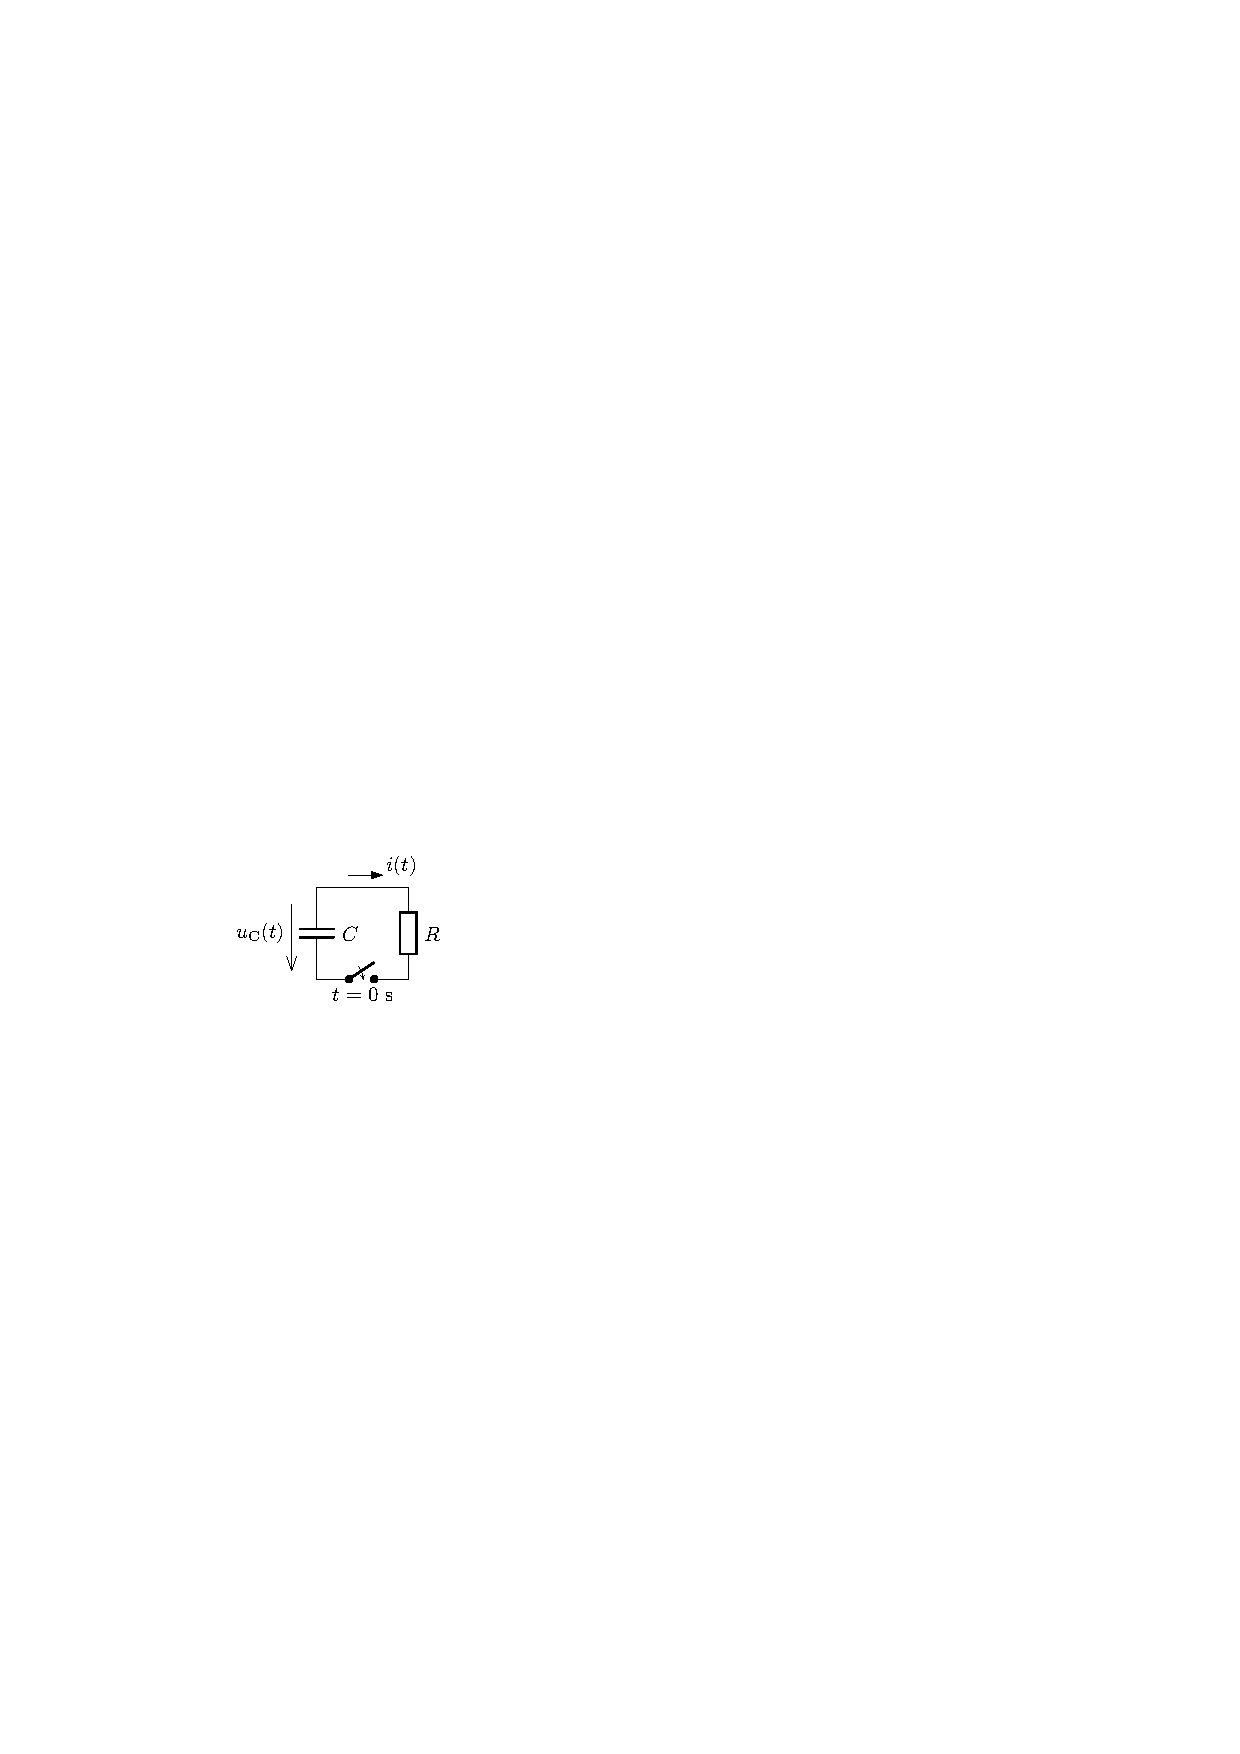
\includegraphics[]{prechodne_jevy/prvni_rad/rc.pdf}
\caption{Obvod prvního řádu s rezistorem a kapacitorem}
\label{fig:prvni_rad_rc}
\end{figure}
Kapacitor je nabit na napětí $U_\mathrm{CO}$, předpokládáme počáteční podmínku ve tvaru
$$
u_c(0-) = u_c(0+) = U_\mathrm{CO}.
$$
S využitím napěťového Kirchhoffova zákona lze zapsat napětí v uzavřené smyčce 
$$
Ri + u_\mathrm{C} = 0.
$$
Proud obvodem lze vyjádřit ve tvaru 
$$
i = C \frac{\dif u_\mathrm{C}}{\dif t}.
$$
Diferenciální rovnice popisující časový průběh proudu v obvodu je
\begin{equation}
RC \frac{\dif u_\mathrm{C}}{\dif t} + u_\mathrm{C} = 0.
\label{eq:prvni_rad_rc_dif_rce}
\end{equation}
Řešení diferenciální rovnice sestává z obecného $u_o$ a partikulárního řešení $u_p$
$$
u_\mathrm{C} = u_o + u_p.
$$
Řešení obecné diferenciální rovnice (rovnice s nulovou pravou stranou) předpokládáme ve tvaru
$$
u_o = K \cdot \me^{\lambda t},
$$
kde $K$ a $\lambda$ jsou neznámé konstanty. Konstantu $\lambda$ získáme řešením charakteristické rovnice k diferenciální rovnici (\ref{eq:prvni_rad_rc_dif_rce})
$$
RC \cdot \lambda + 1 = 0.
$$
Převrácenou hodnotu řešení charakteristické rovnice $\lambda = - \frac{1}{RC}$
$$
\tau = - \frac{1}{\lambda} = RC
$$ 
nazýváme časovou konstantou. 

Partikulární řešení představuje ustálený stav. Je zřejmé, že po odeznění přechodného děje bude kapacitor plně vybit
$$
u_p = u_\mathrm{C}(\infty) = 0.
$$
Napětí na kapacitoru získáme jako součet obecného a partikulárního řešení ve tvaru
$$
u_\mathrm{C} = u_o + u_p = K \cdot \me^{-\frac{t}{RC}}.
$$
Aplikujeme počáteční podmínku napětí na kapacitoru $u_c(0+) = U_\mathrm{CO}$
$$
U_\mathrm{CO} = K \cdot \lim_{t \rightarrow 0} \left( \me^{-\frac{t}{RC}} \right) = K
$$
a ihned získáme neznámou konstantu $K = U_\mathrm{CO}$. Časový průběh napětí na kapacitoru $u_c(t)$ je zobrazen na obrázku \ref{fig:prvni_rad_rc_graf_u} a lze vyjádřit ve tvaru
\begin{equation}
u_\mathrm{C} = U_\mathrm{CO} \cdot \me^{-\frac{t}{RC}}.
\label{eq:prvni_rad_rc_u}
\end{equation}
\begin{figure}[h!]
\centering
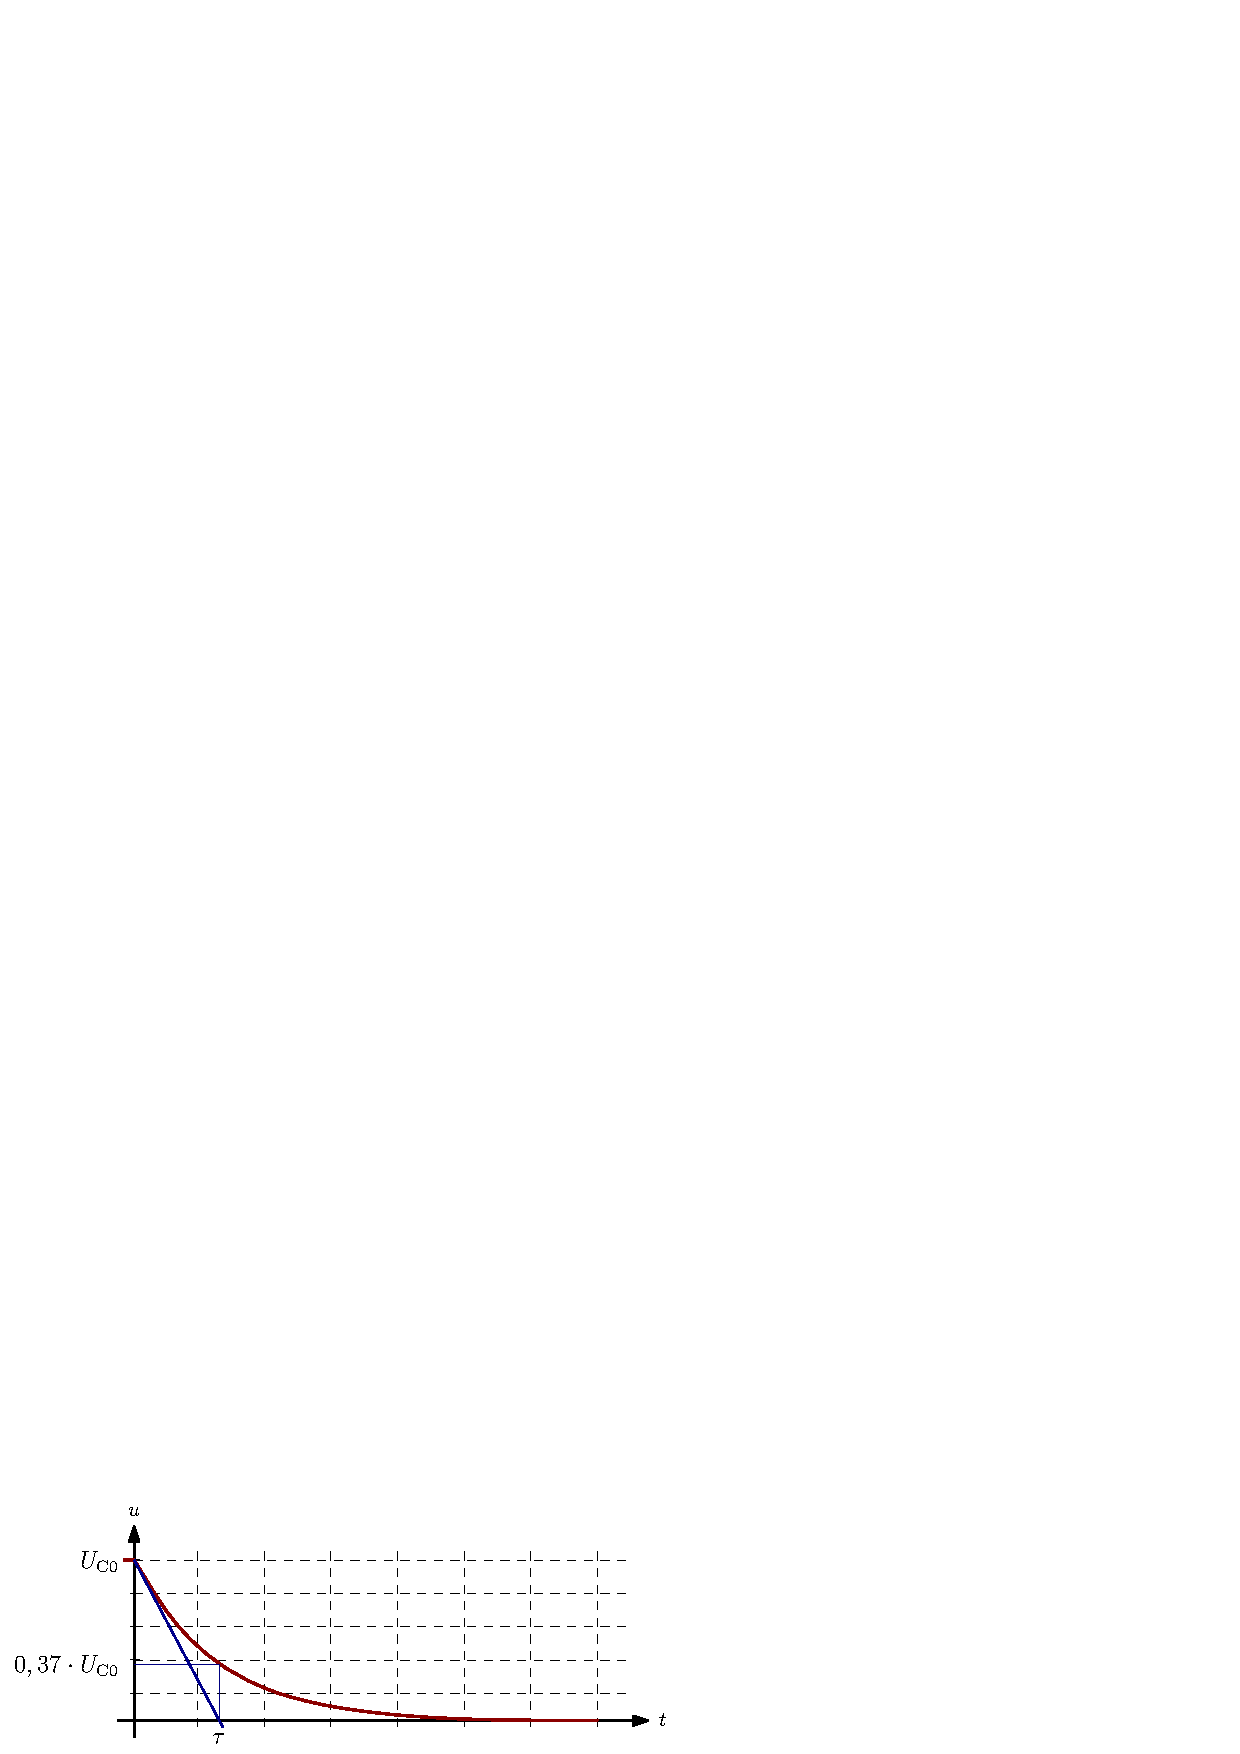
\includegraphics[]{prechodne_jevy/prvni_rad/rc_graf_u.pdf}
\caption{Časový průběh napětí na kapacitoru}
\label{fig:prvni_rad_rc_graf_u}
\end{figure}
Proud obvodem je vidíme na obrázku \ref{fig:prvni_rad_rc_graf_i} a získáme ho derivací napětí na kapacitoru
$$
i = C \frac{\dif u_\mathrm{C}}{\dif t} = - \frac{U_\mathrm{CO}}{R} \cdot \me^{-\frac{t}{RC}}.
$$
\begin{figure}[h!]
\centering
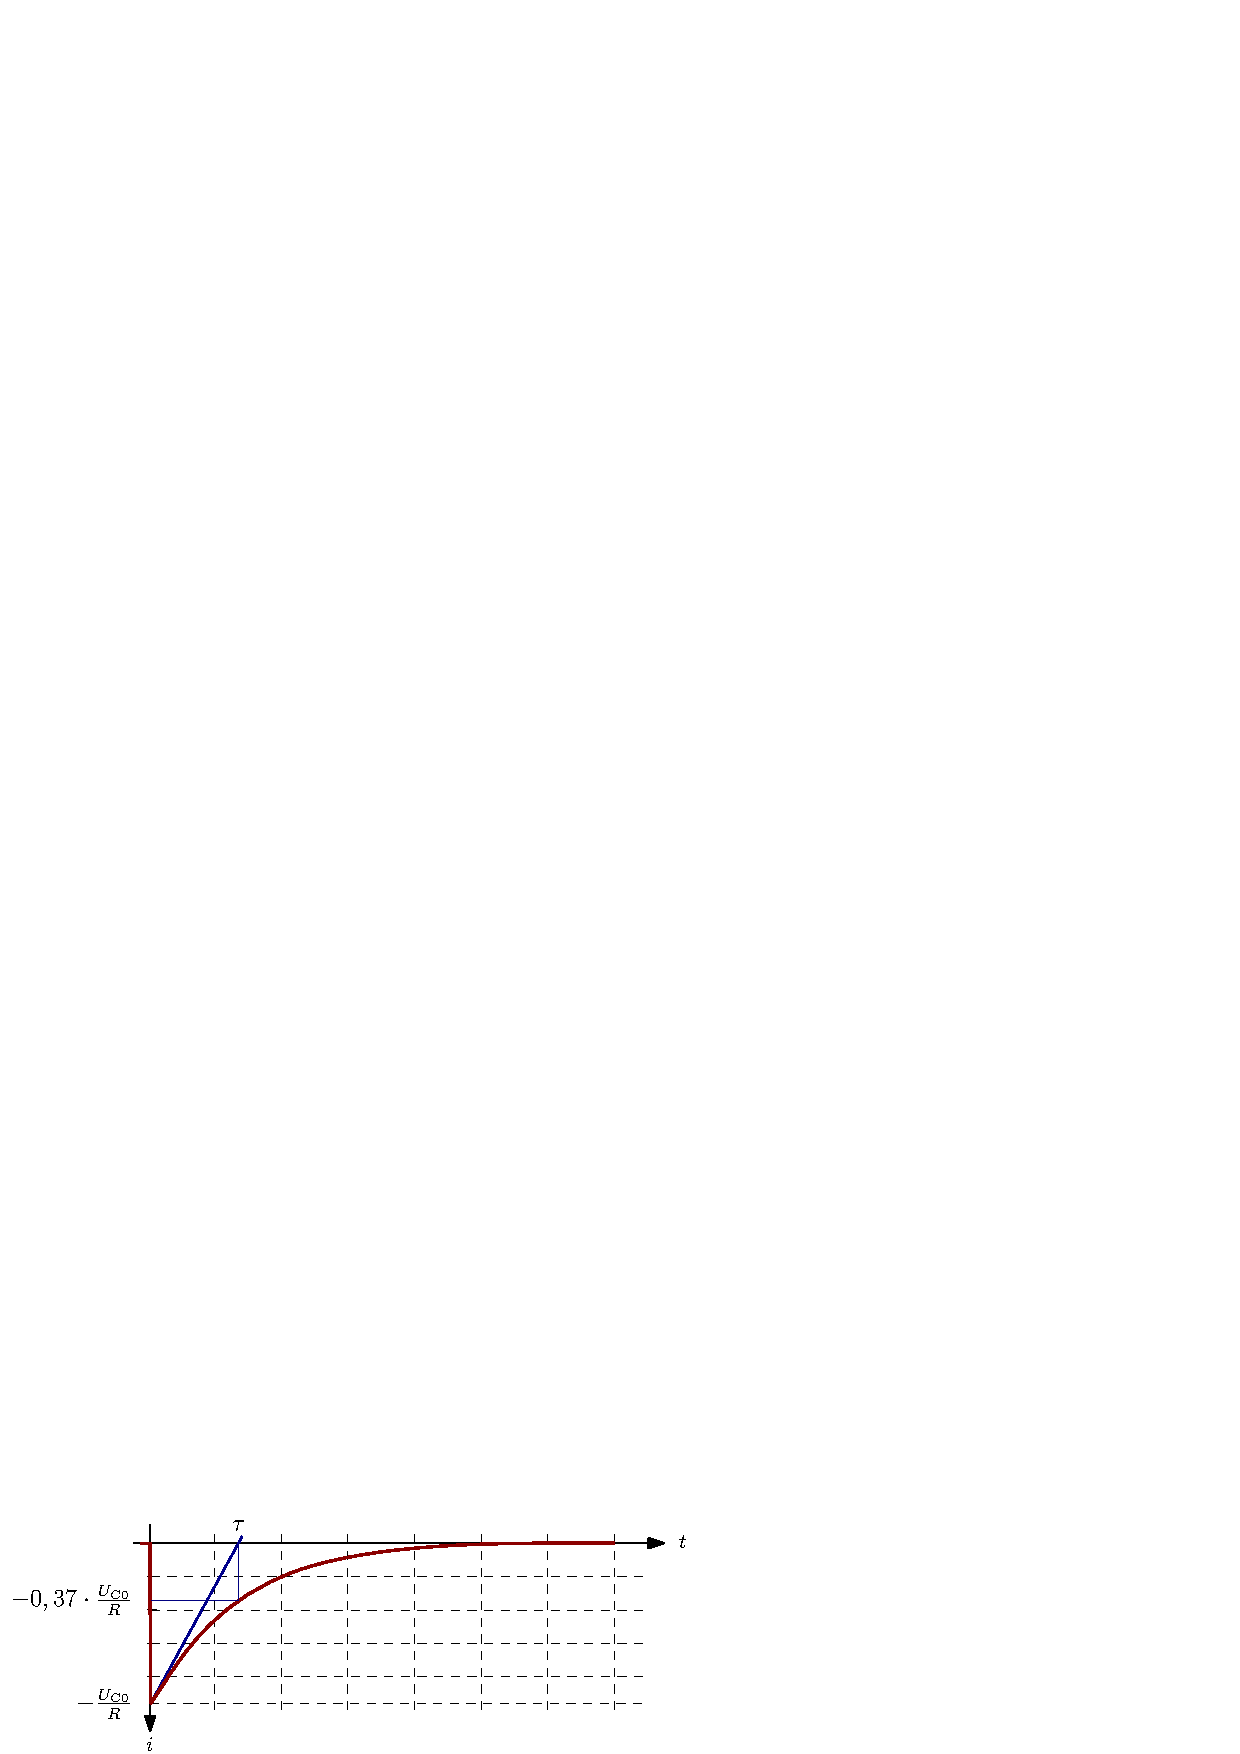
\includegraphics[]{prechodne_jevy/prvni_rad/rc_graf_i.pdf}
\caption{Časový průběh proudu v obvodu}
\label{fig:prvni_rad_rc_graf_i}
\end{figure}

Význam časové konstanty je patrný z následující úvahy. Nejprve dosadíme za čas do vztahu (\ref{eq:prvni_rad_rc_u}) časovou konstantu $\tau$ a získáme
$$
u_\mathrm{C}(\tau) = U_\mathrm{CO} \cdot \me^{-\frac{\tau}{\tau}} = U_\mathrm{CO} \cdot \me^{-1} = 0,368 \cdot U_\mathrm{CO}.
$$
Je zřejmé, že za dobu jedné časové konstanty klesne napětí na kapacitoru na 37 \% napětí na počátku přechodného děje. Z obrázku \ref{fig:prvni_rad_rc_graf_tau} je patrný vliv velikosti časové konstant na rychlost přechodného děje. Menší hodnota časové konstanty způsobí rychlejší dosažení ustáleného stavu. Obvod můžeme považovat za ustálený za dobu $5\tau$ kdy napětí klesne na 0,7~\% své původní hodnoty.
\begin{figure}[h!]
\centering
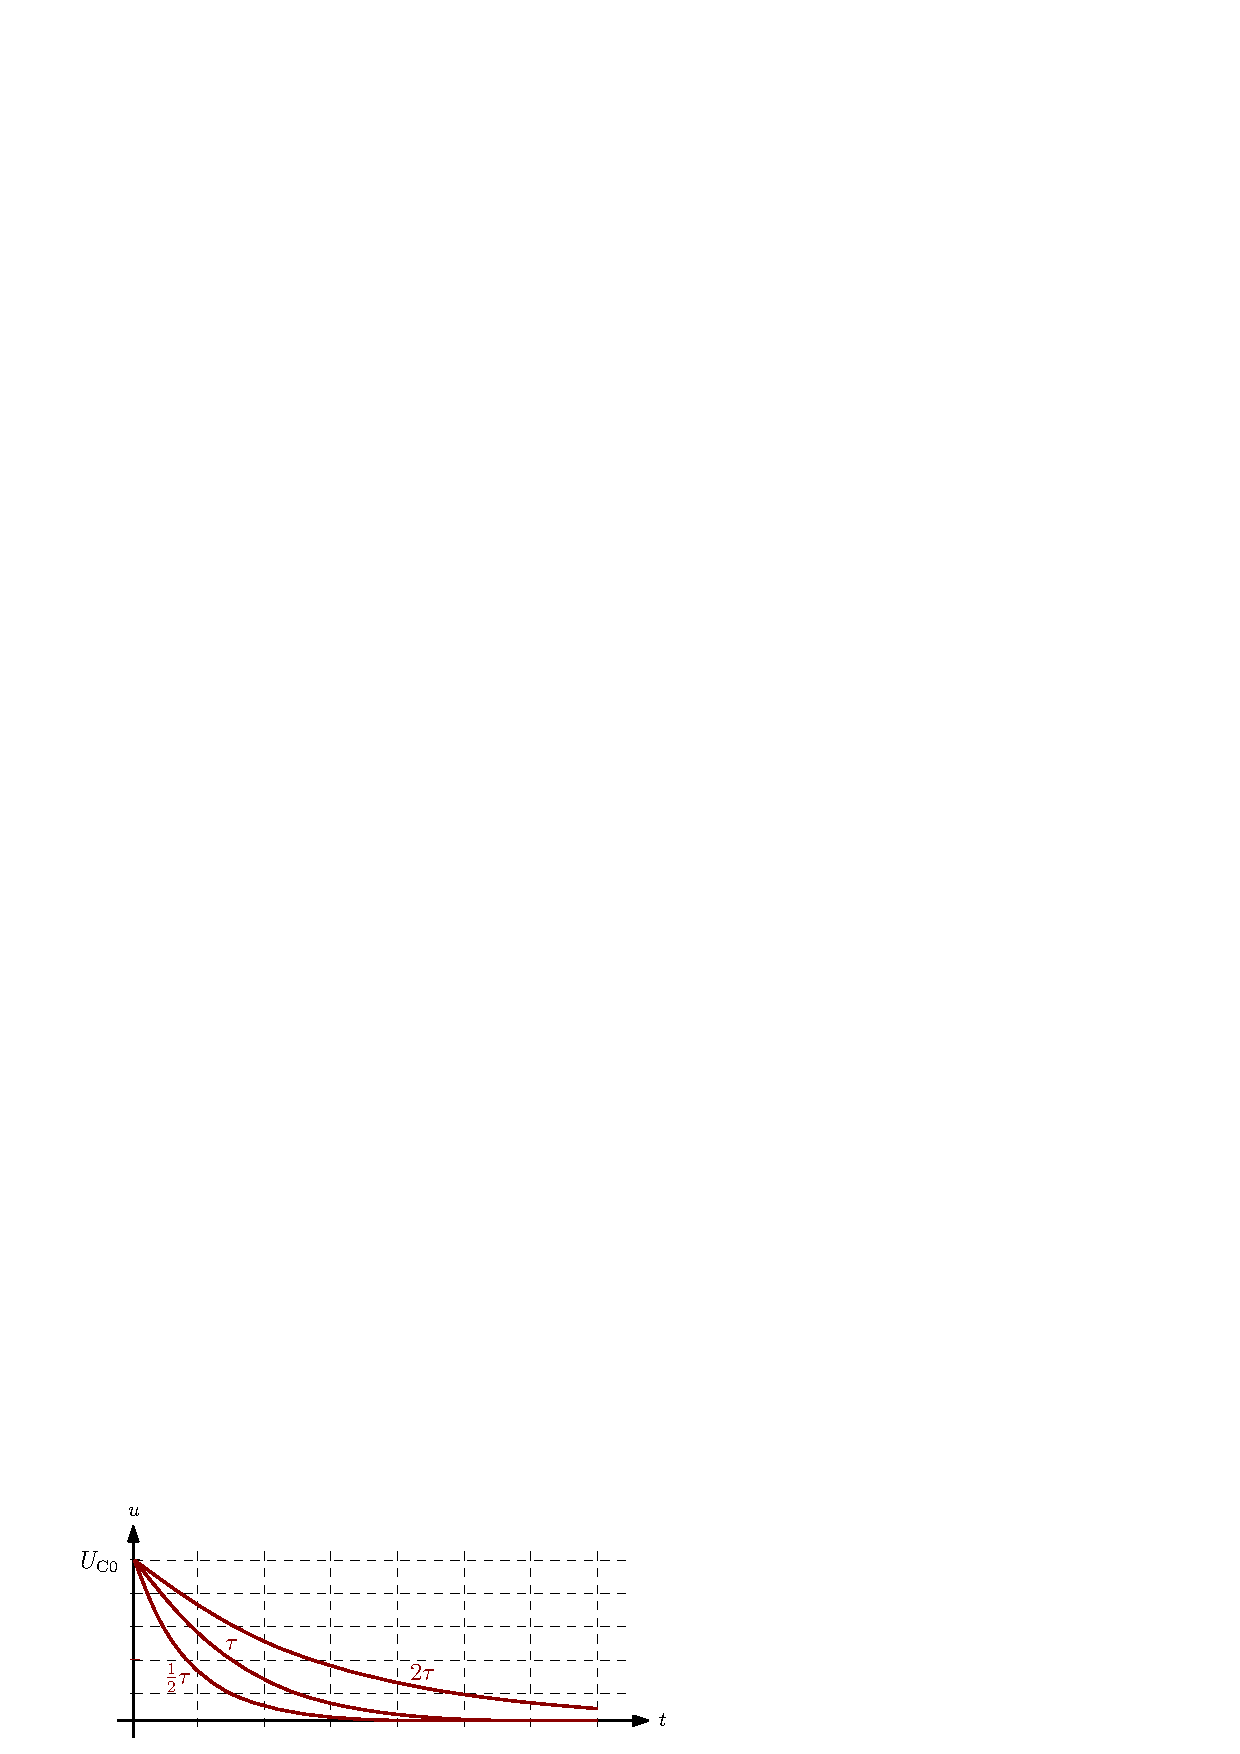
\includegraphics[]{prechodne_jevy/prvni_rad/rc_graf_tau.pdf}
\caption{Vliv časové konstanty na rychlost přechodného děje}
\label{fig:prvni_rad_rc_graf_tau}
\end{figure}

\subsubsection{Sériový RL obvod}

Uvažujme elektrický obvod na obrázku \ref{fig:prvni_rad_rl} tvořený rezistorem $R$ a induktorem $L$ napájený zdrojem napětí $U_0$. 
\begin{figure}[h!]
\centering
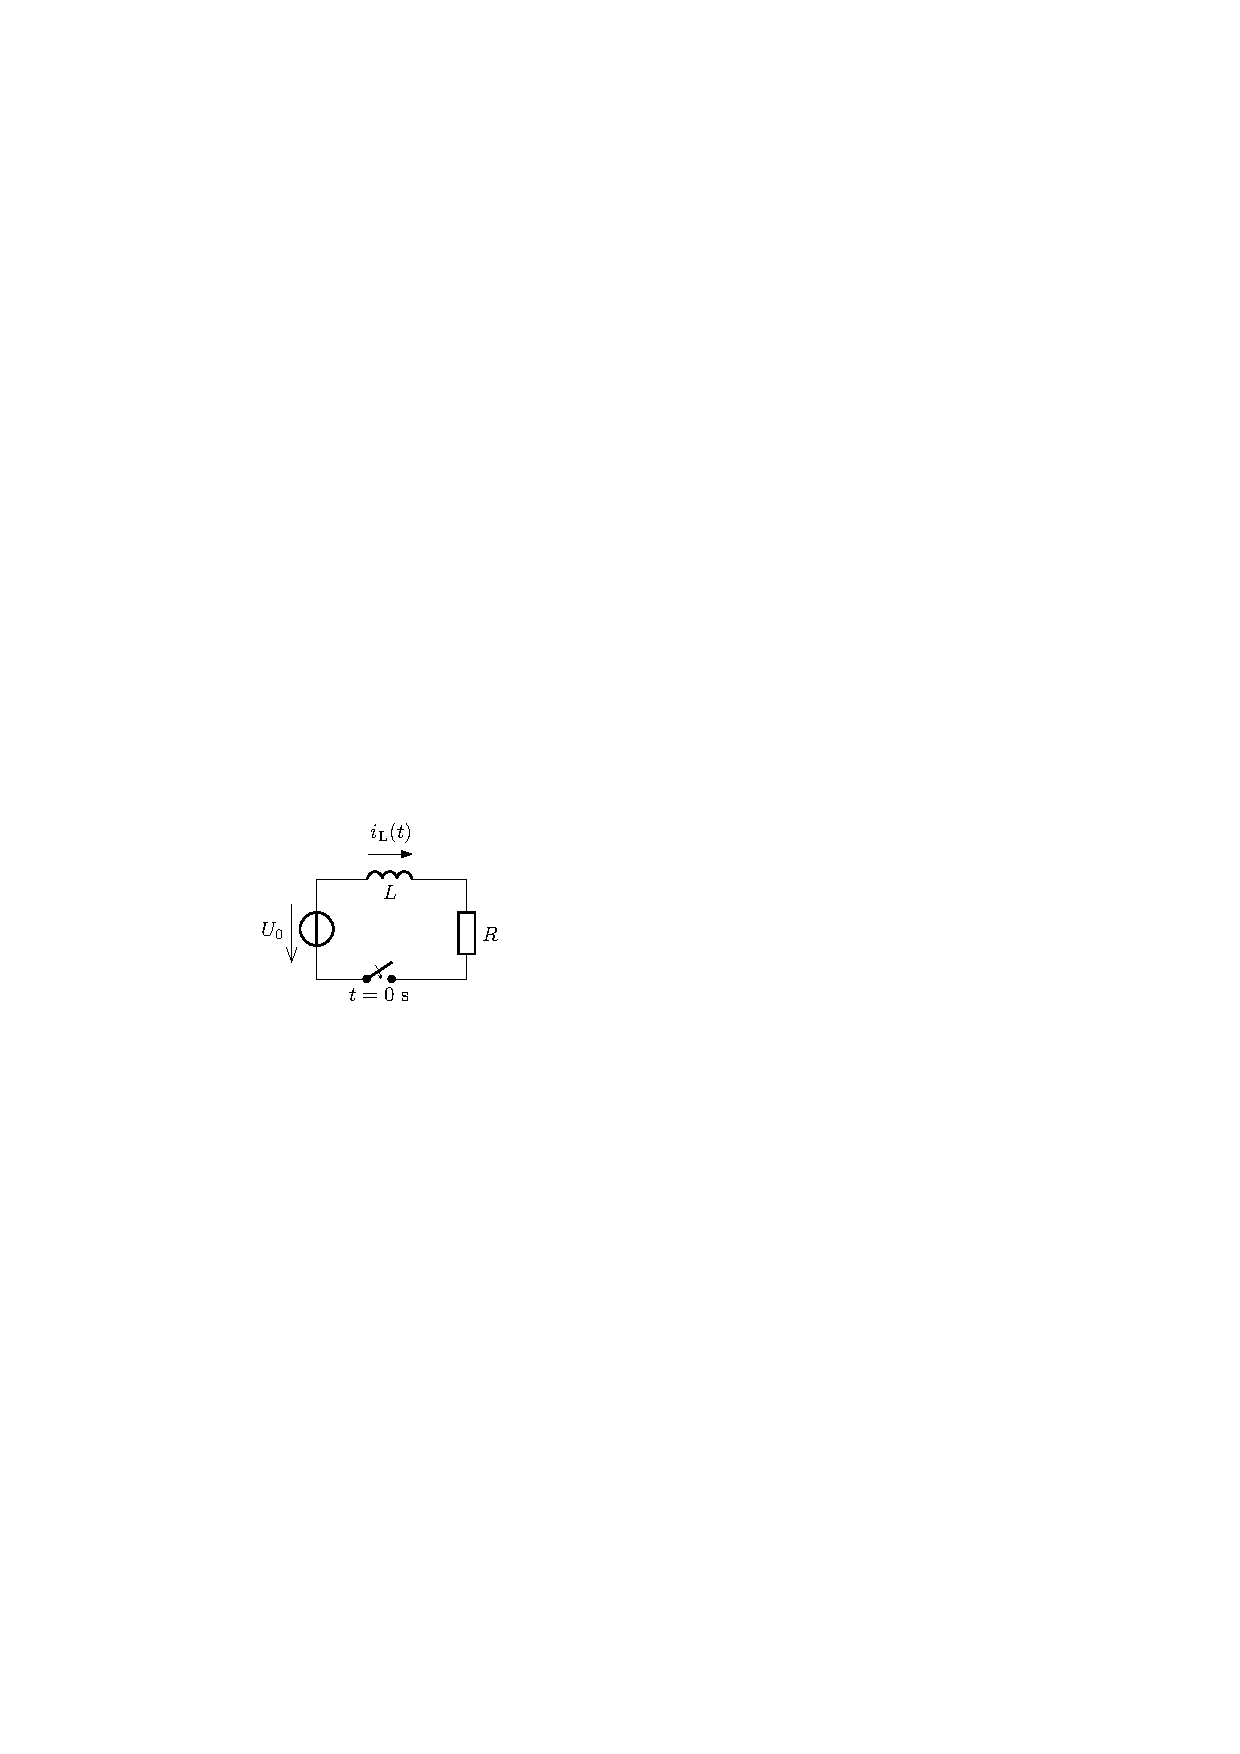
\includegraphics[]{prechodne_jevy/prvni_rad/rl.pdf}
\caption{Obvod prvního řádu s rezistorem a induktorem}
\label{fig:prvni_rad_rl}
\end{figure}

\begin{figure}[h!]
\centering
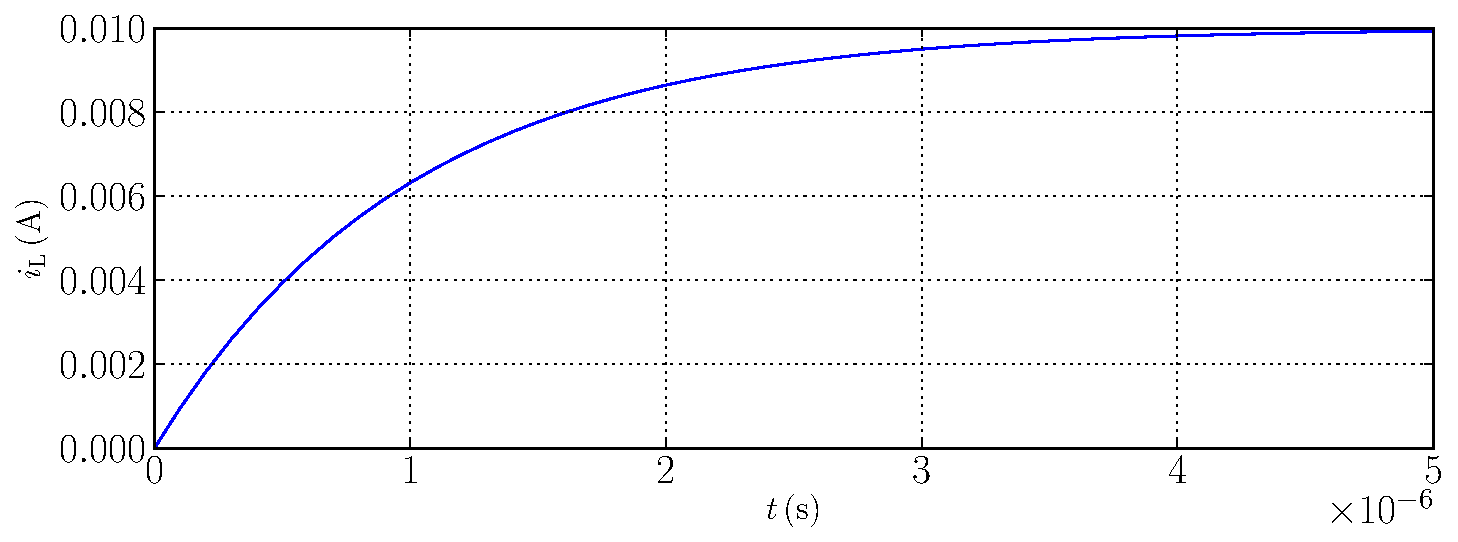
\includegraphics[width=13cm]{prechodne_jevy/prvni_rad/obvod_rl_proud.pdf}
\caption{Sériový RL obvod: proud induktorem}
\label{fig:obvod_rl_proud}
\end{figure}

\section{Přechodné jevy druhého řádu}

Uvažujme sériový elektrický obvod na obrázku \ref{fig:druhy_rad_rlc} tvořený rezistorem $R$, induktorem $L$ a kapacitorem $C$ napájený stejnosměrným zdrojem o napětí $U_0$. 
\begin{figure}[h!]
\centering
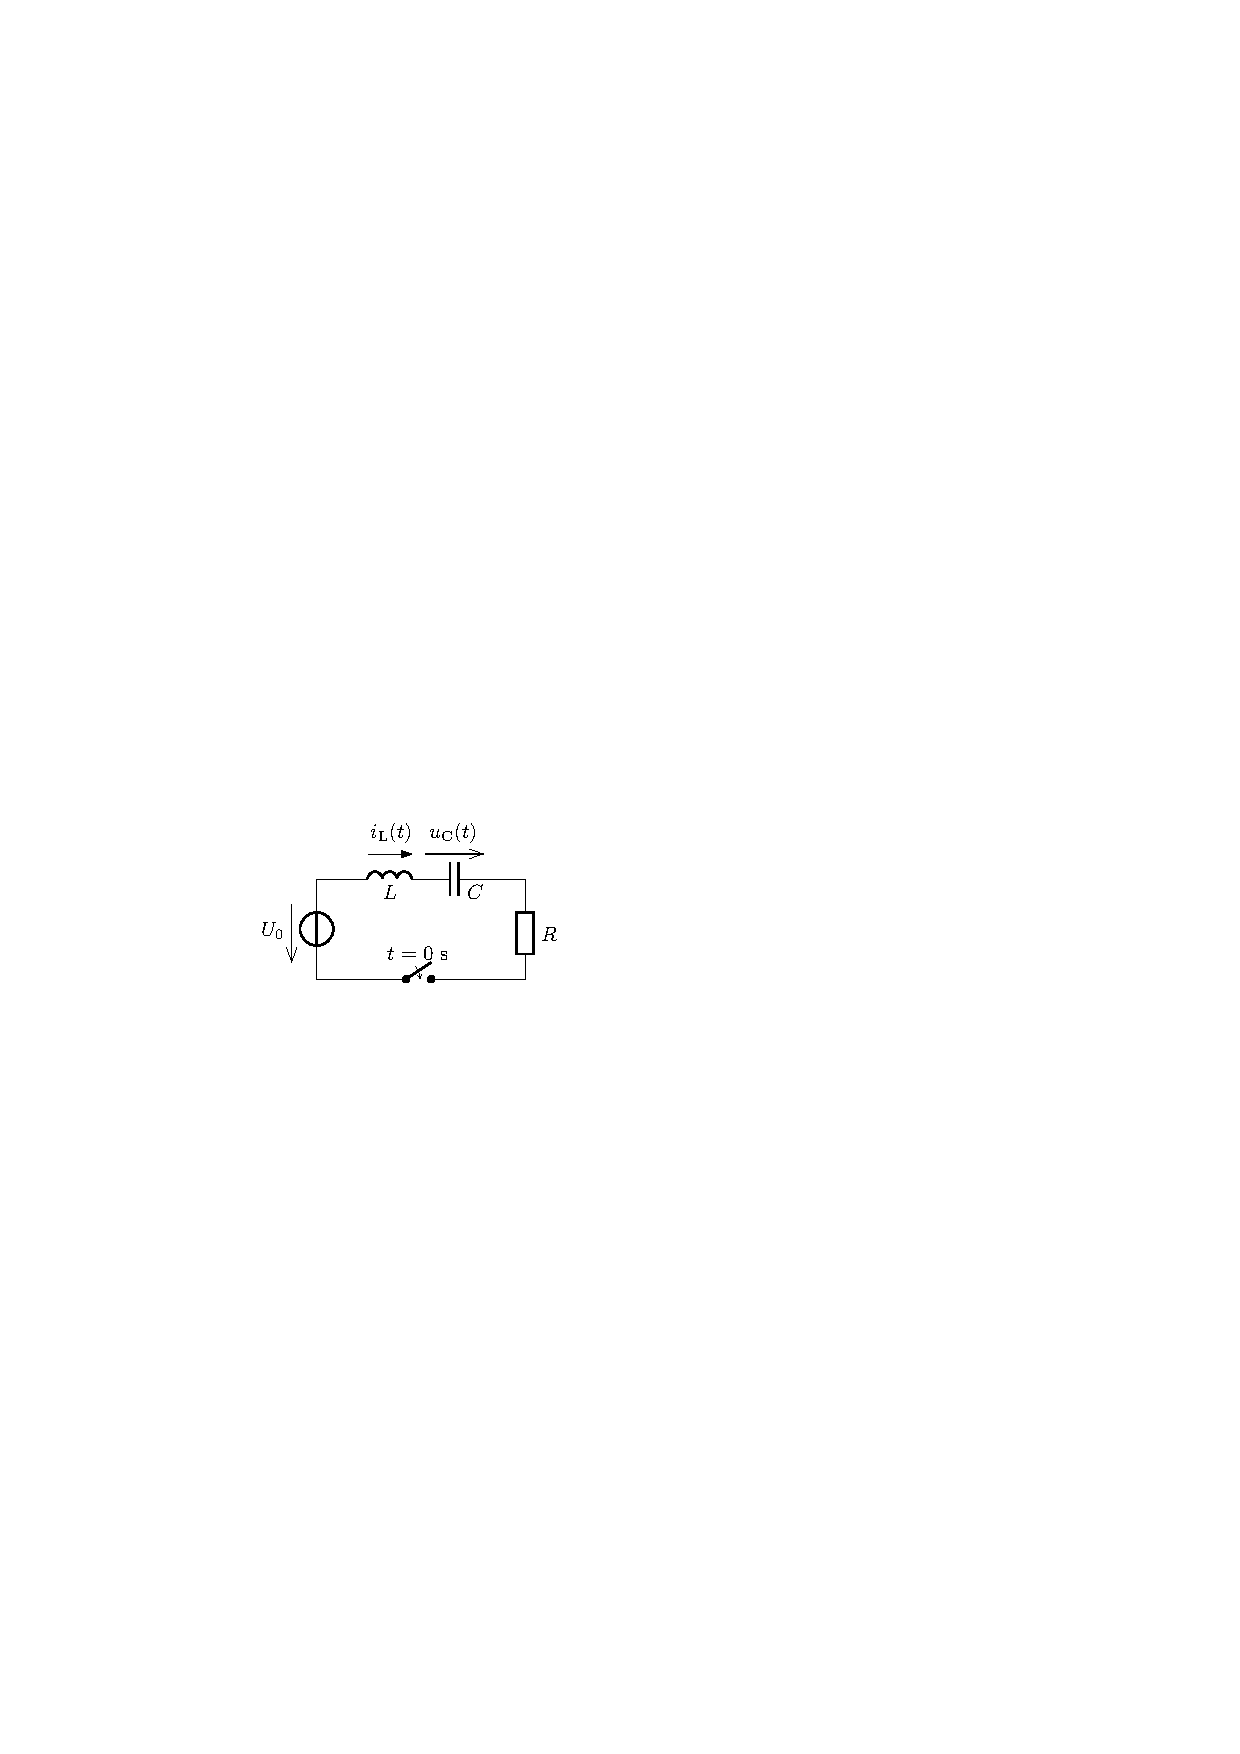
\includegraphics[]{prechodne_jevy/druhy_rad/rlc.pdf}
\caption{Sériová obvod druhého řádu}
\label{fig:druhy_rad_rlc}
\end{figure}
Vyjdeme opět z napěťového Kirchhoffova zákona. Součet napětí na jednotlivých prvcích obvodu je roven napětí zdroje
$$
u_\mathrm{R} + u_\mathrm{L} + u_\mathrm{C} = U_0
$$
Napětí na rezistoru, induktoru a kapacitoru vyjádříme
$$
u_\mathrm{R} = Ri_\mathrm{L} = RC \frac{\dif u_\mathrm{C}}{\dif t},~~~~~
u_\mathrm{L} = L \frac{\dif i_\mathrm{L}}{\dif t} = LC \frac{\dif^2 u_\mathrm{C}}{\dif t^2},~~~~~u_\mathrm{C} = u_\mathrm{C}
$$
Po dosazení získáme diferenciální rovnici pro napětí na kapacitoru $u_\mathrm{C}$ ve tvaru
$$
\frac{\dif^2 u_\mathrm{C}}{\dif t^2} + \frac{R}{L} \cdot \frac{\dif u_\mathrm{C}}{\dif t} + \frac{1}{LC} \cdot u_\mathrm{C} = \frac{U_0}{LC}.
$$
Diferenciální rovnici můžeme ovšem rovněž odvodit pro proud induktorem $i_\mathrm{L}$ s využitím následujících vztahů
$$
u_\mathrm{R} = Ri_\mathrm{L},~~~~~
u_\mathrm{L} = L \frac{\dif i_\mathrm{L}}{\dif t} ,~~~~~u_\mathrm{C} = \frac{1}{C} \int_o^t i_\mathrm{L} \dif t
$$
Získáme
$$
Ri_\mathrm{L} + L \frac{\dif i_\mathrm{L}}{\dif t} + \frac{1}{C} \int_o^t i_\mathrm{L} \dif t = U_0.
$$
Uvedenou rovnici můžeme derivovat a po jednoduché úpravě dostaneme
$$
\frac{\dif^2 i_\mathrm{L}}{\dif t^2} + \frac{R}{L} \cdot \frac{\dif i_\mathrm{L}}{\dif t} + \frac{1}{LC} \cdot i_\mathrm{L} = 0.
$$
Uvažujeme nulové počáteční podmínky. Napětí na kapacitoru bylo na počátku děje nulové
$$
u_\mathrm{C}(0+) = 0.
$$
Proud induktorem byl rovněž nulový
$$
i_\mathrm{L}(0+) = C \frac{\dif u_\mathrm{C}}{\dif t} \left( 0+ \right) = 0
$$
Řešení diferenciální rovnice sestává z obecného $u_o$ a partikulárního řešení $u_p$
$$
u_\mathrm{L} = u_o + u_p.
$$
Nejprve se zaměříme na řešení homogenní rovnice. Charakteristickou rovnici k uvedené diferenciální rovnici (napěťové i proudové) lze zapsat ve tvaru kvadratické rovnice
$$
\lambda^2 + \frac{R}{L} \lambda + \frac{1}{LC} = 0
$$
s kořeny
$$
\lambda_{1,2} = -\frac{R}{2L} \pm \sqrt{\left( \frac{R}{2L} \right)^2 - \frac{1}{LC}}.
$$
S využitím substituce $\beta = \frac{R}{2L}$ a $\omega_0 = \frac{1}{\sqrt{LC}}$ zapíšeme rovnici ve tvaru
$$
\lambda_{1,2} = -\beta \pm \sqrt{\beta^2 - \omega_0^2} = -\beta \pm \alpha,
$$
kde $\omega_0$ je rezonanční frekvence obvodu a konstantu $\beta$ lze interpretovat jako činitel tlumení. 

Rozeznáváme tři stavy RLC obvodu:
\begin{enumerate*}
\item $\beta > \omega_0$, aperiodický děj,
\item $\beta = \omega_0$, obvod na mezi aperiodicity,
\item $\beta < \omega_0$, kmitavý děj.
\end{enumerate*}
Kritický odpor $R_\mathrm{k}$, při kterém se obvod nachází na mezi aperiodicity, lze vyjádřit z podmínky
$$
\beta = \omega_0~~~ \rightarrow ~~~\left( \frac{R_\mathrm{k}}{2L} \right)^2 = \frac{1}{LC}~~~ \rightarrow ~~~R_\mathrm{k} = 2 \sqrt{\frac{L}{C}}.
$$
Partikulárním řešením je ustálený stav. Kapacitor bude po odeznění přechodného děje nabit na napětí zdroje a obvodem nebude procházet žádný proud 
$$
u_\mathrm{C}(\infty) = U_0,~~~~~~
i_\mathrm{L}(\infty) = 0.
$$

\subsubsection{Aperiodický děj}

V případě kladného diskriminantu ($\beta > \omega_0$) hovoříme o aperiodickém ději. Kořeny charakteristické rovnice $\lambda_{1,2}$ jsou kladná reálná čísla. Řešení diferenciální rovnice předpokládáme ve tvaru součtu dvou exponenciálních funkcí
$$
u_\mathrm{C} = K_1 \cdot \me^{\lambda_1 t} + K_2 \cdot \me^{\lambda_2 t} + U_0.
$$
Časové konstanty lze zapsat ve tvaru
$$
\tau_1 = - \frac{1}{\lambda_1} = \frac{1}{\beta - \alpha},~~~~~
\tau_2 = - \frac{1}{\lambda_2} = \frac{1}{\beta + \alpha},~~~~~
\tau_2 > \tau_1
$$
Pro dosazení počátečních podmínek, je nejprve nutné provést časovou derivaci uvedené rovnice 
$$
\frac{\dif u_\mathrm{C}}{\dif t} = K_1 \lambda_1 \cdot \me^{\lambda_1 t} + K_2 \lambda_2 \cdot \me^{\lambda_2 t}.
$$
Po dosazení počátečních podmínek dostame dvě algebraické rovnice
$$
K_1 + K_2 + U_0 = 0
$$
a
$$
K_1 \lambda_1 + K_2 \lambda_2 = 0
$$
Jejich řešením získáme konstanty $K_1$ a $K_2$. Proud kapacitorem je úměrný časové derivaci napětí
$$
i_\mathrm{L} = i_\mathrm{C} = C \frac{\dif u_\mathrm{C}}{\dif t} = C \left( K_1 \lambda_1 \cdot \me^{\lambda_1 t} + K_2 \lambda_2 \cdot \me^{\lambda_2 t} \right).
$$

\subsubsection{Obvod na mezi aperiodicity}

V případě nulového diskriminantu ($\beta = \omega_0$) hovoříme o ději na mezi aperiodicity. Kořen charakteristické rovnice $\lambda_{1,2}$ je dvojný a je jím kladné reálné číslo $\lambda = - \frac{R}{2L} = - \beta$. Řešení diferenciální rovnice předpokládáme ve tvaru
$$
u_\mathrm{C} = \left( K_1 + K_2 t \right) \me^{\lambda t} + U_0.
$$
Časovou konstantu lze zapsat ve tvaru
$$
\tau = - \frac{1}{\lambda} = \frac{1}{\beta}.
$$
Časová derivace uvedené diferenciální rovnice 
$$
\frac{\dif u_\mathrm{C}}{\dif t} = \left( K_1 \lambda + K_2 \lambda t + K_2 \right) \me^{\lambda t}.
$$
Po aplikaci počátečních podmínek dostame dvě algebraické rovnice
$$
K_1 + U_0 = 0
$$
a
$$
K_1 \lambda + K_2 = 0
$$
Jejich řešením získáme konstanty $K_1$ a $K_2$. Proud kapacitorem je úměrný časové derivaci napětí
$$
i_\mathrm{L} = i_\mathrm{C} = C \frac{\dif u_\mathrm{C}}{\dif t} = C \left( K_1 \lambda + K_2 \lambda t + K_2 \right) \me^{\lambda t} .
$$

\subsubsection{Kmitavý děj}

V případě záporného diskriminantu ($\beta < \omega_0$) hovoříme o kmitavém ději. Kořeny charakteristické rovnice $\lambda_{1,2}$ jsou komplexně sdružená čísla a lze je zapsat ve tvaru
$$
\lambda_{1,2} = - \beta \pm \mj \omega_\mathrm{d},
$$
kde parametr $\omega_\mathrm{d} = \alpha = \sqrt{\beta^2 - \omega_0^2}$ nazýváme frekvence vlastních kmitů. Řešení diferenciální rovnice předpokládáme opět ve tvaru
$$
u_\mathrm{C} = K_1 \cdot \me^{\left( - \beta + \mj \omega_\mathrm{d} \right) t} + K_2 \cdot \me^{\left(- \beta - \mj \omega_\mathrm{d} \right) t} + U_0 = \me^{- \beta t} \left( K_1 \cdot \me^{\mj \omega_\mathrm{d} t} + K_2 \cdot \me^{- \mj \omega_\mathrm{d} t} \right) + U_0.
$$
S využitím Eulerovy identity
$$
\me^{\mj \varphi} = \cos \varphi + \mj \sin \varphi,~~~~~
\me^{- \mj \varphi} = \cos \varphi - \mj \sin \varphi.
$$
dostaneme řešení ve tvaru
$$
u_\mathrm{C} = \me^{- \beta t} \left[ K_1 \left( \cos \omega_\mathrm{d} t + \mj \sin \omega_\mathrm{d} t \right) + K_2 \left( \cos \omega_\mathrm{d} t - \mj \sin \omega_\mathrm{d} t \right) \right] + U_0 =
$$
$$
= \me^{- \beta t} \left[ \left( K_1 + K_2 \right) \cos \omega_\mathrm{d} t + \mj \left( K_1 - K_2 \right) \sin \omega_\mathrm{d} t \right] + U_0.
$$
Z uvedeného vztahu je patrné, že napětí na kapacitoru bude kmitat s periodou $T~=~\frac{2 \pi}{\omega_\mathrm{d}}$ a dále bude exponenciálně tlumené. Konstanty $K_1$ a $K_2$ opět získáme dosazením počátečních podmínek.

Na obrázku \ref{fig:obvod_rlc_napeti} je zobrazen průběh napětí na kapacitoru v případě aperiodického děje, kmitavého děje a děje v obvodu na mezi aperiodicity. Obrázek \ref{fig:obvod_rlc_proud} zobrazuje průběh proudu v obvodu.

\begin{figure}[h!]
\centering
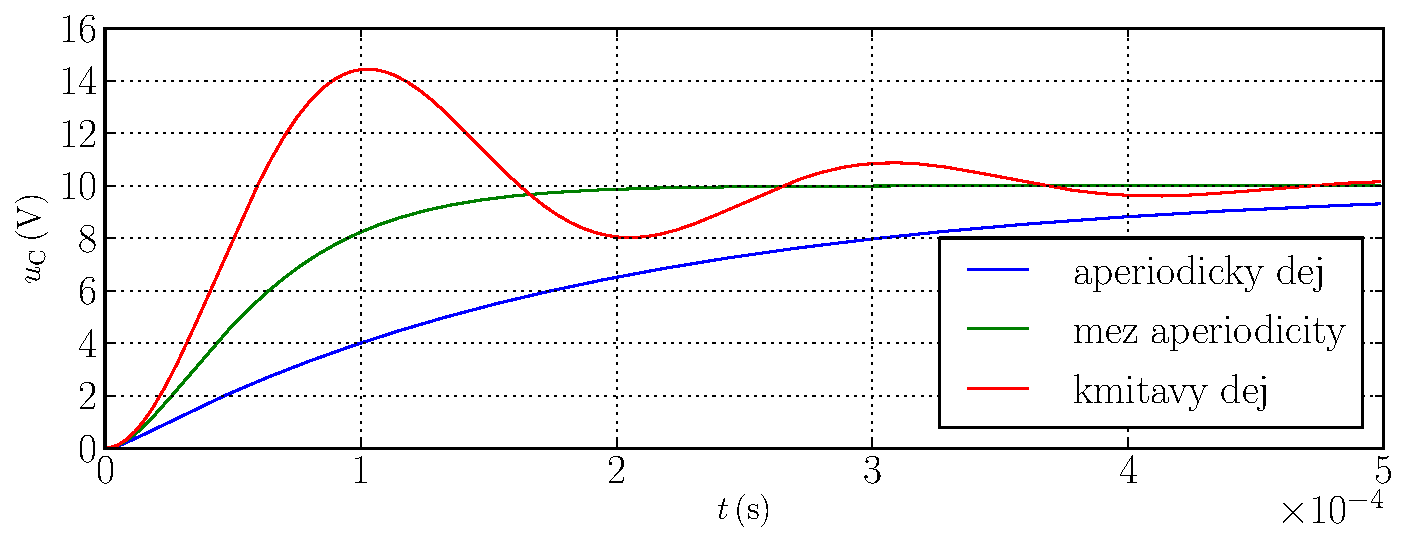
\includegraphics[width=13cm]{prechodne_jevy/druhy_rad/obvod_rlc_napeti.pdf}
\caption{Sériový RLC obvod: napětí na kapacitoru}
\label{fig:obvod_rlc_napeti}
\end{figure}

\begin{figure}[h!]
\centering
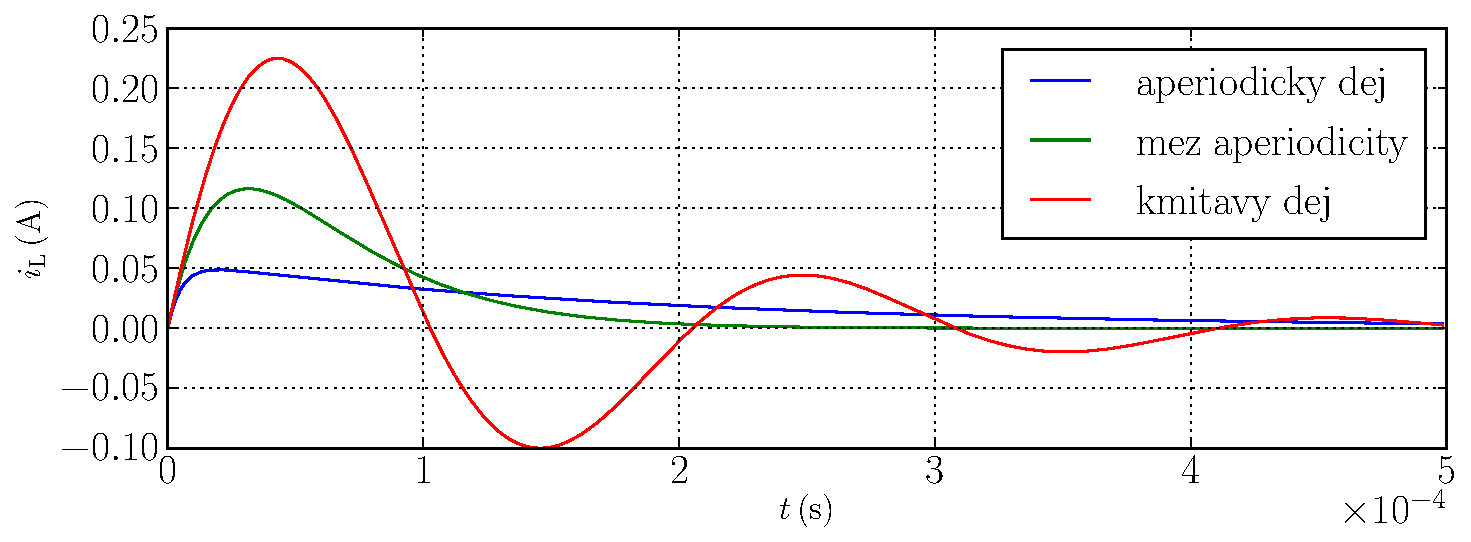
\includegraphics[width=13cm]{prechodne_jevy/druhy_rad/obvod_rlc_proud.pdf}
\caption{Sériový RLC obvod: proud induktorem}
\label{fig:obvod_rlc_proud}
\end{figure}

\subsubsection{Netlumený kmitavý děj}

Speciálním případem kmitavého děje je netlumený kmitavý děj, který nastane při nulovém tlumení obvodu $\beta = 0$. Nutno poznamenat, že tento jev je ideální případ při nulové rezistivitě odporu $R$.

\subsection{Příklady}

Uvažujte obvod dle obrázku \ref{fig:druhy_rad_priklad_1} napájený stejnosměrným zdrojem s napětím $U_0 = 10~\mathrm{V}$ s následujícími parametry: $R_1 = 40~\mathrm{\Omega}$, $R_2 = 40~\mathrm{\Omega}$, $L = 0,4~\mathrm{H}$ a $C = 30~\mathrm{\mu F}$. Vyšetřete průběh proudu $i_\mathrm{L}$ induktorem. Před přechodným dějem se obvod nachází v ustáleném stavu.
\begin{figure}[h!]
\centering
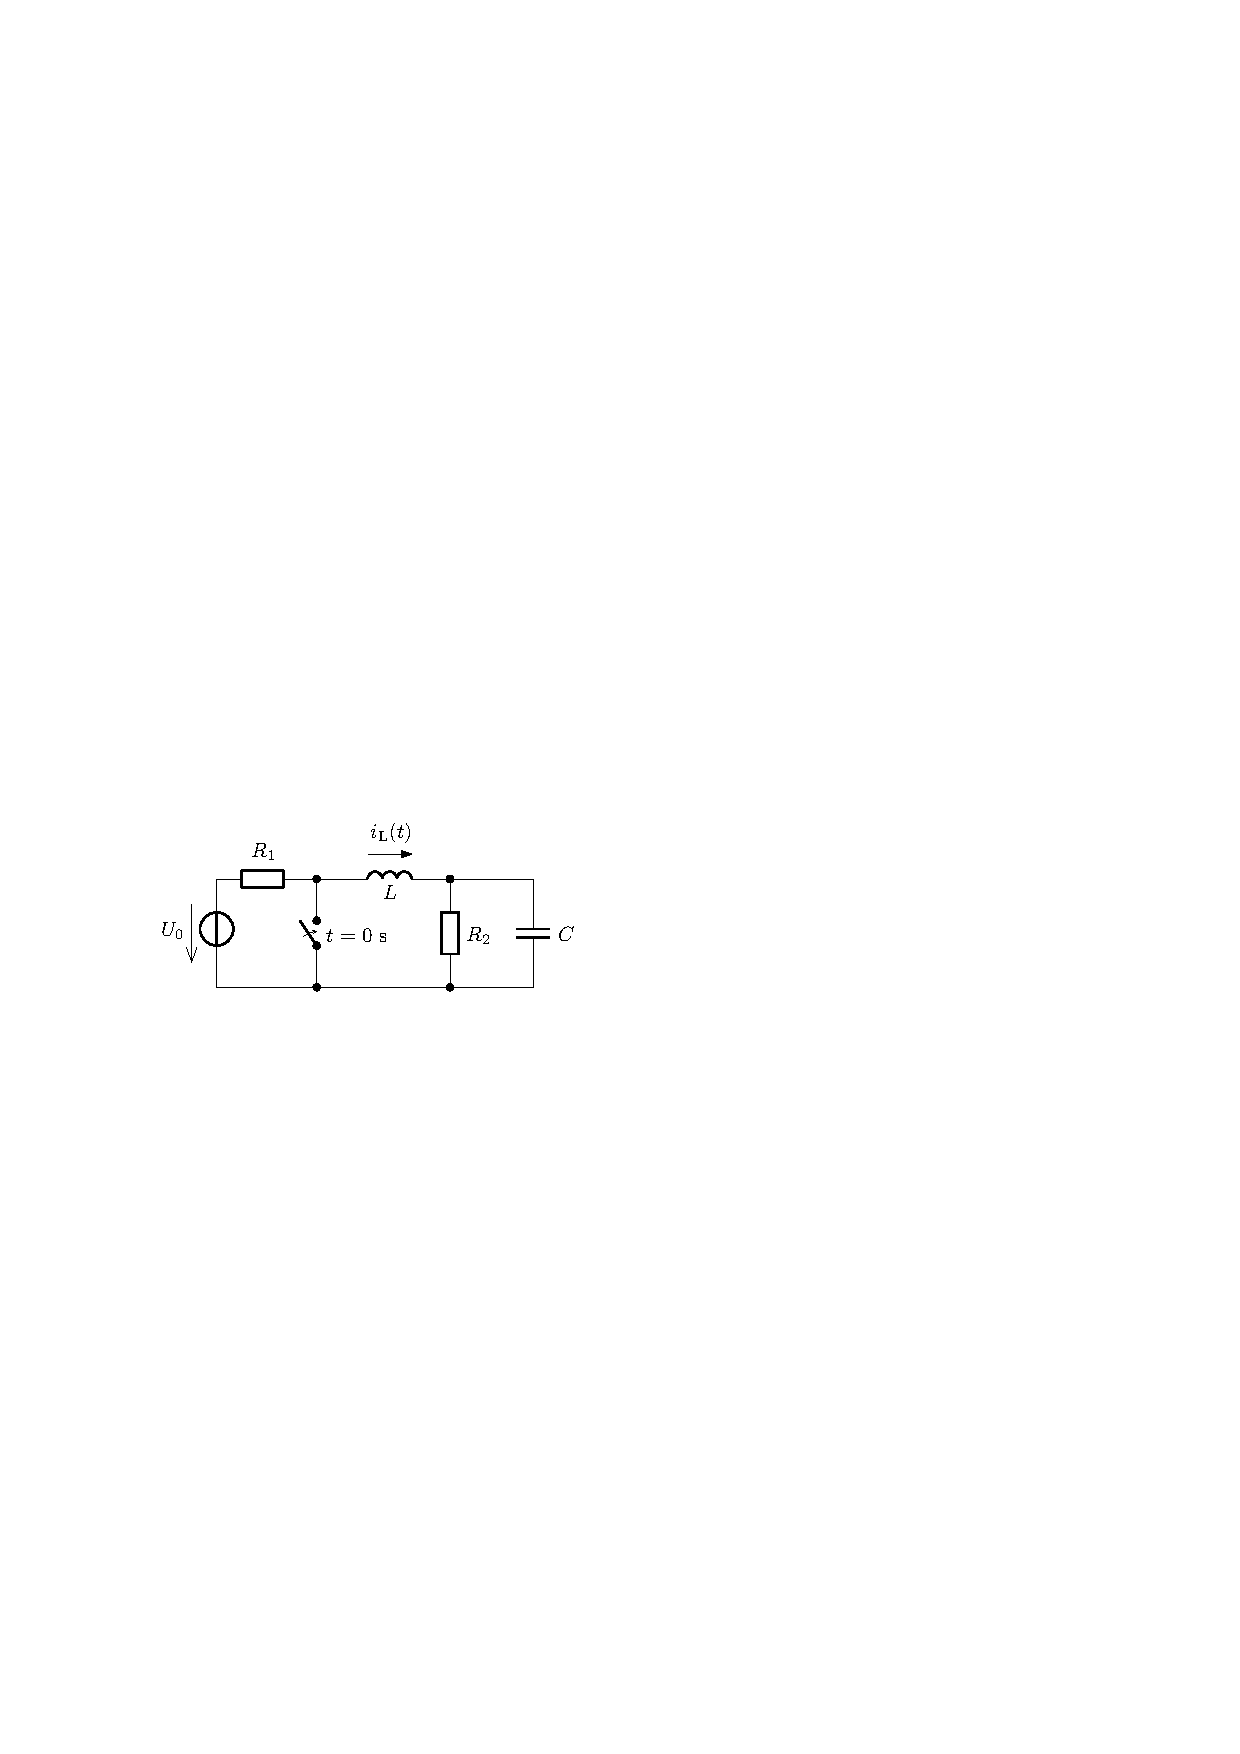
\includegraphics[]{prechodne_jevy/druhy_rad/priklad_1.pdf}
\caption{Obvod druhého řádu}
\label{fig:druhy_rad_priklad_1}
\end{figure}

\section{Obvody buzené časově proměnnými zdroji}

\subsection{Sériový RL obvod buzený harmonický zdrojem}

\begin{figure}[h!]
\centering
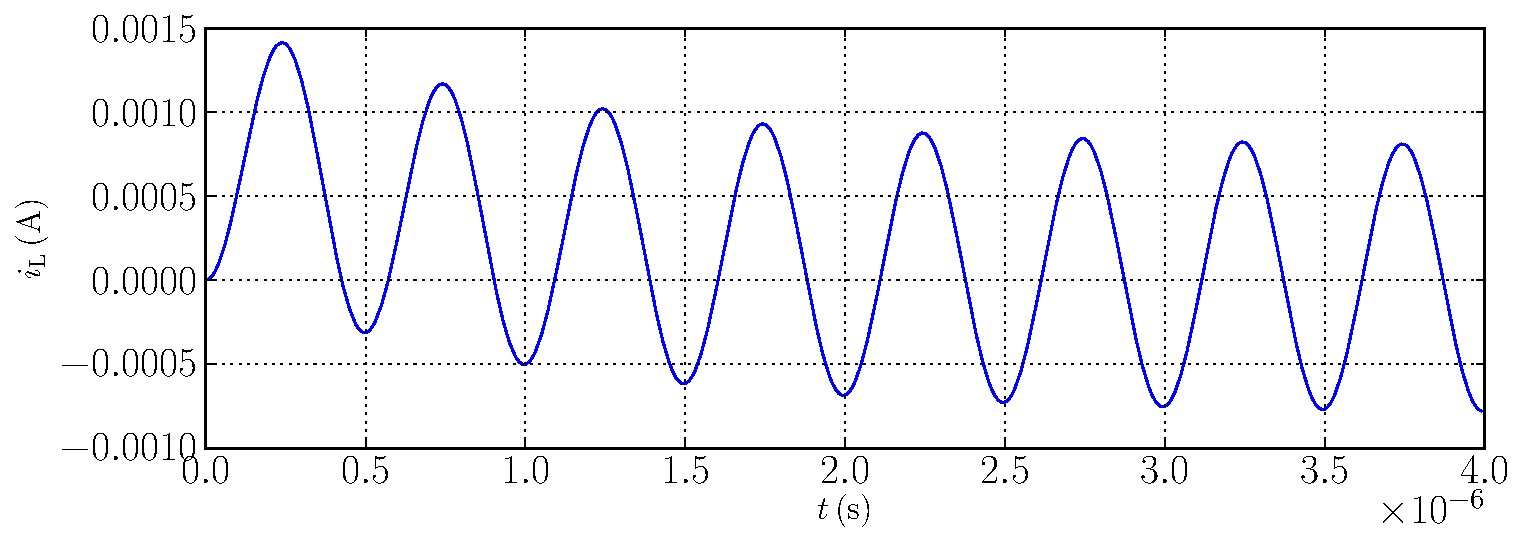
\includegraphics[width=13cm]{prechodne_jevy/prvni_rad/obvod_rl_harmonicky_proud.pdf}
\caption{Sériový RL obvod: proud induktorem}
\label{fig:obvod_rl_proud}
\end{figure}

\section{Metoda stavových proměnných}



%\chapter{Nelineární obvody}
%\section{Úvod}
%\section{Analýza nelineárních obvodů}

%\chapter{Stacionární elektromagnetické pole}
%\section{Základní veličiny a vlastnosti}
%\section{Elektrostatické pole}

\subsection{Coulombův zákon}

\subsection{Kapacita}
%\section{Elektrické proudové pole}
%\section{Magnetické obvody}
%\section{Energie stacionárního elektromagnetického pole}

\bibliographystyle{unsrt}
%\bibliography{bib_world}

% \listoffigures
% \listoftables

\appendix

% \chapter{Vektorová analýza -- diferenciální a~integrální operátory}
% \section{Kartézský souřadnicový systém}
\label{appendix:vektorova_analyza}

Složky libovolného vektoru jsou v~obecném případě funkcí souřadnic a~času. Nejprve ukážeme tvary operátorů v~kartézském souřadnicovém systému $x, y, z$ s~příslušnými jednotkovými vektory $\mathbf{i}$, $\mathbf{j}$ a~$\mathbf{k}$.

\begin{figure}[!hbt]
\centering
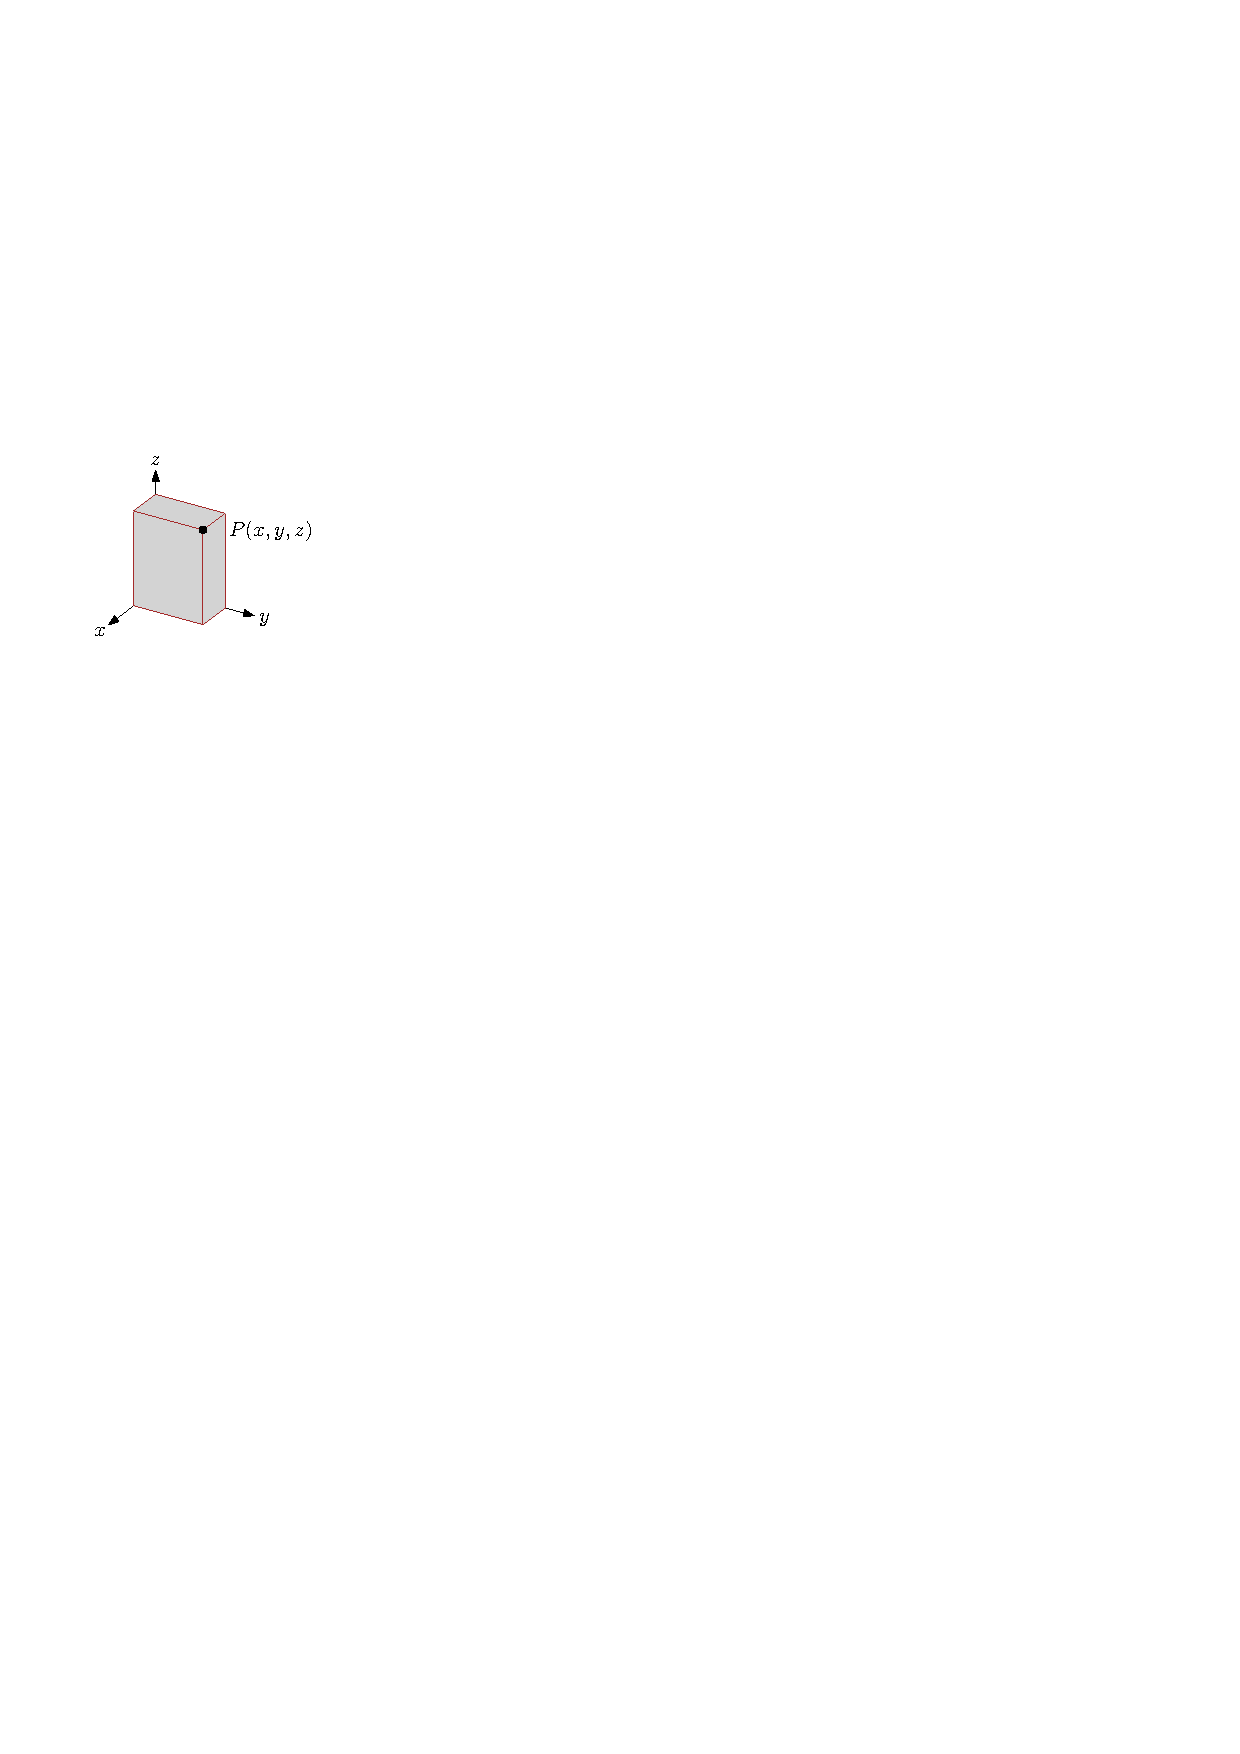
\includegraphics[]{prilohy/vektorova_analyza/kartezsky.pdf}
\caption{Kartézský souřadnicový systém}
\label{fig:vektorova_analyza_kartezsky}
\end{figure}

Zavedeme operátor „nabla“ -- $\nabla$, který je definován jako
$$
\nabla = \mathbf{i}\,\frac{\partial}{\partial x} + \mathbf{j}\,\frac{\partial}{\partial y} + \mathbf{k}\,\frac{\partial}{\partial z}\,.
$$
Pomocí tohoto operátoru lze jednoduše nadefinovat všechny tři důležité diferenciální operátory: gradient, divergenci a~rotaci.

\subsection*{Gradient}

Gradient skalární funkce $\varphi$ lze vyjádřit ve tvaru
$$
\grad \varphi = \nabla\varphi\ = \mathbf{i}\,\frac{\partial \varphi}{\partial x} + \mathbf{j}\,\frac{\partial \varphi}{\partial y} + \mathbf{k}\,\frac{\partial \varphi}{\partial z}\,.
$$

\subsection*{Divergence}

Divergence vektorového pole $\vec A(x, y, z)$ zapíšeme jako

$$
\div \vec A = \nabla \cdot \vec A = \frac{\partial A_x}{\partial x} + \frac{\partial A_y}{\partial y} + \frac{\partial A_z}{\partial z}
$$
kde $A_x$, $A_y$ a~$A_z$ jsou složky vektorové funkce $\vec A(x, y, z)$.

\subsection*{Rotace}

Rotaci vektorového pole $\vec A(x, y, z)$ definujeme výrazem
$$
\vec A = \nabla \times \vec A = 
\left|
\begin{array}{ccc}
  \mathbf{i} & \mathbf{j} & \mathbf{k} \\
  \frac{\partial}{\partial x} & \frac{\partial}{\partial y} & \frac{\partial}{\partial z} \\
  A_x & A_y & A_z
\end{array}
\right|\,.
$$

\subsection*{Laplaceův operátor}

Operátor $\nabla^2$ (nebo také $\triangle$) se nazývá Laplaceův operátor a~lze vyjádřit ve tvaru
$$
\nabla^2 = \triangle = \frac{\partial^2}{\partial x^2}+\frac{\partial^2}{\partial y^2}+
\frac{\partial^2}{\partial z^2}.
$$
Může působit na skalární nebo vektorovou funkci
$$
\nabla^2 \varphi = \triangle \varphi = \frac{\partial^2\varphi}{\partial x^2}+\frac{\partial^2\varphi}{\partial y^2}+
\frac{\partial^2\varphi}{\partial z^2},
$$
$$
\triangle\, \vec A = \frac{\partial^2 \vec A}{\partial x^2} + \frac{\partial^2 \vec A}{\partial y^2} + 
\frac{\partial^2 \vec A}{\partial z^2}.
$$
Laplaceův operátor splňuje Laplaceovu rovnici. 

\subsection*{Operátor rot rot}

Jeden z~často používaných operátorů je rot rot. V~případě kartézského systému souřadnice je snadné odvodit vztah
$$
\rot \rot \vec A = \grad \div \vec A - \triangle\,\vec A.
$$

\section{Válcový souřadnicový systém}

Válcový souřadnicový systém je definován vztahy
$$
x = r\cos \alpha,\ \ y = r \sin \alpha,\ \ z = z,\ \ \alpha \in \langle 0,2\pi \rangle.
$$

\begin{figure}[!hbt]
\centering
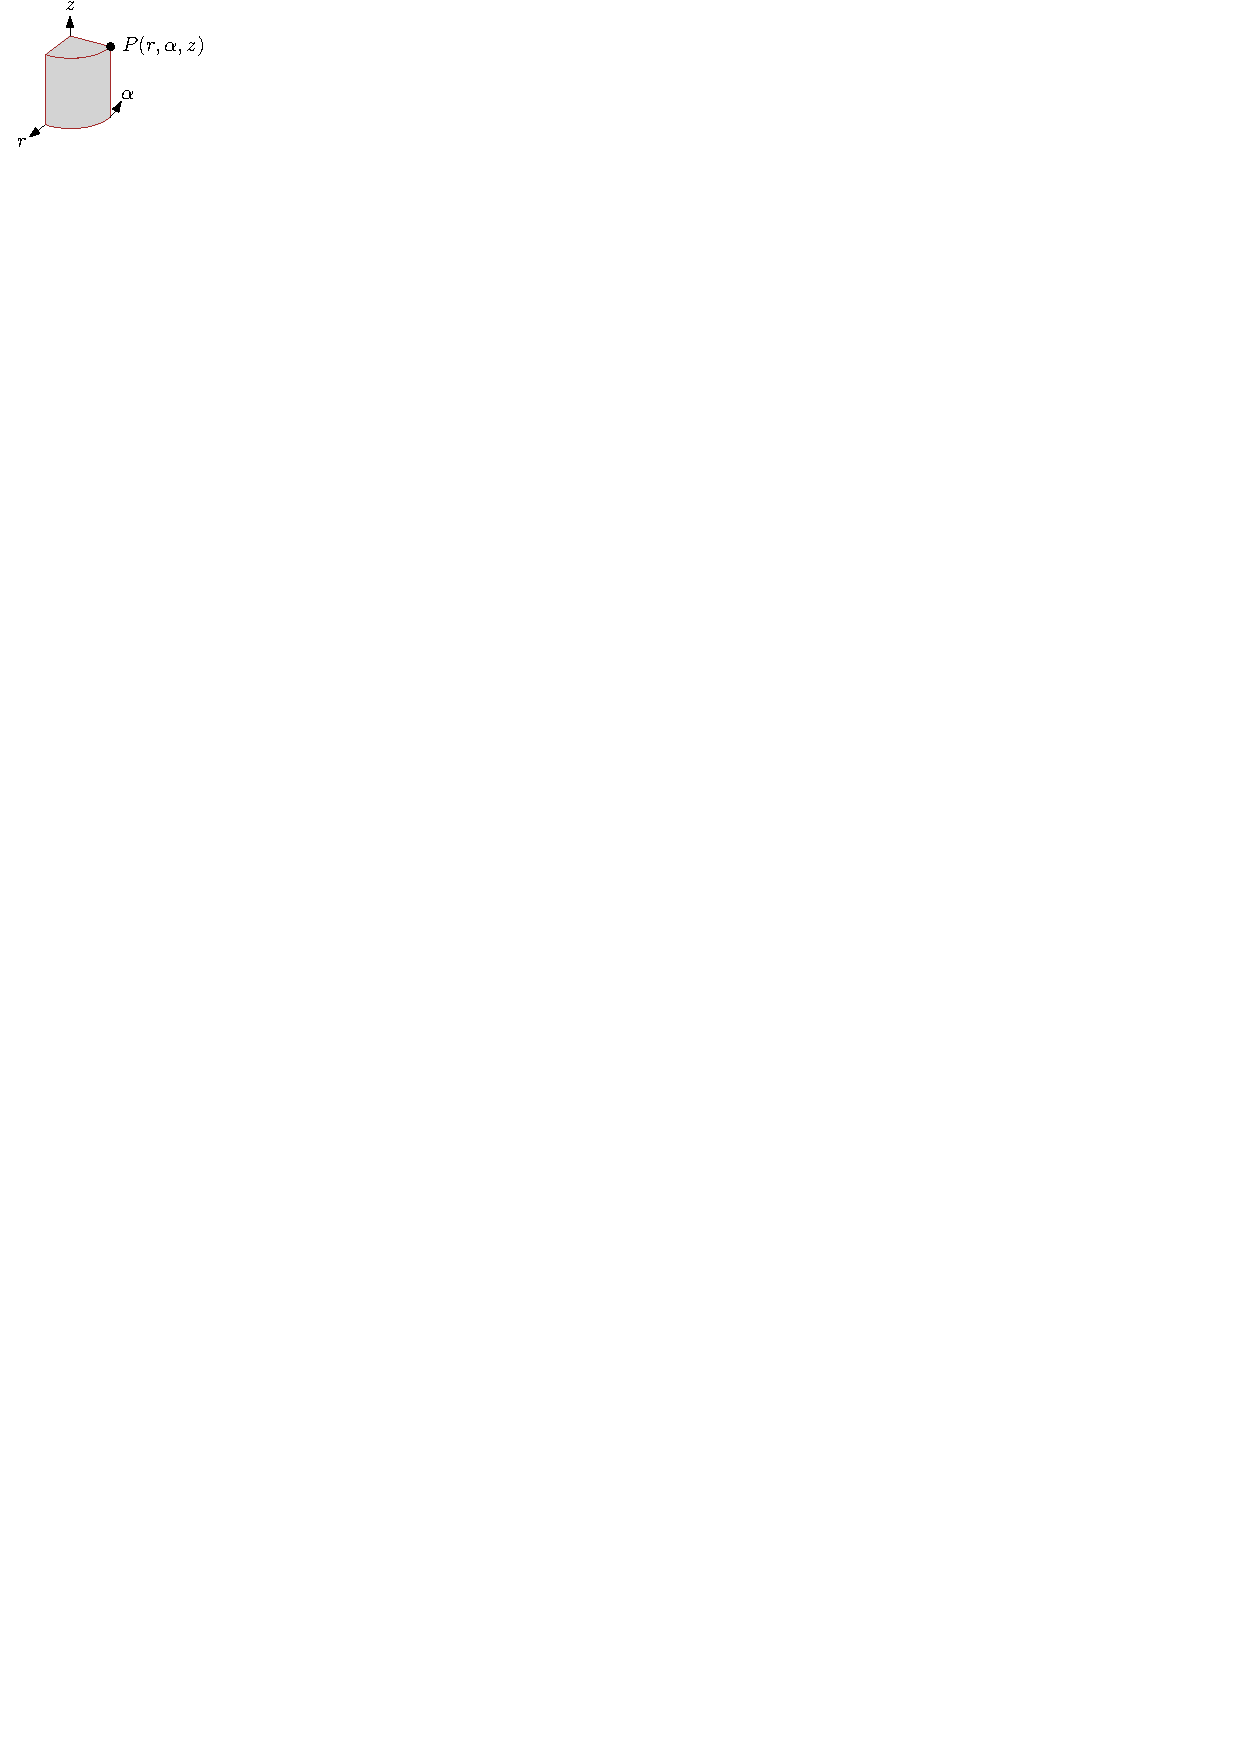
\includegraphics[]{prilohy/vektorova_analyza/valcovy.pdf}
\caption{Válcový souřadnicový systém}
\label{fig:vektorova_analyza_valcovy}
\end{figure}

Příslušné diferenciální operátory gradient, divergence a~rotace lze za použití jednotkových vektorů $\textbf{r}_0$, $\textbf{a}_0$ a~$\textbf{z}_0$ zapsat ve tvaru
$$
\grad \,\varphi=\mbox{\textbf{r}}_0 \frac{\partial\varphi}{\partial r}
+\mbox{\textbf{a}}_0\frac{1}{r}\frac{\partial\varphi}{\partial \alpha}+
\mbox{\textbf{z}}_0\frac{\partial\varphi}{\partial z},
$$
$$
\div \vec A = \frac{1}{r}\frac{\partial (rA_r)}{\partial r}+
\frac{1}{r}\frac{\partial A_\alpha}{\partial \alpha}+\frac{\partial A_z}{\partial z} = 
\frac{\partial A_r}{\partial r} + \frac{A_r}{r} +
\frac{1}{r}\frac{\partial A_\alpha}{\partial \alpha}+\frac{\partial A_z}{\partial z},
$$
$$
\rot \vec A = \frac{1}{r}\cdot
\left|
\begin{array}{ccc}
  \mbox{\textbf{r}}_0 & r\mbox{\textbf{a}}_0 & \mbox{\textbf{z}}_0 \\
  \frac{\partial}{\partial r} & \frac{\partial}{\partial \alpha} & \frac{\partial}{\partial z} \\
  A_r & rA_\alpha & A_z
\end{array}
\right|
$$
a~$$
\triangle = \frac{1}{r}\frac{\partial}{\partial r}\left(r
\frac{\partial}{\partial r}\right) + \frac{1}{r^2}\frac{\partial^2}{\partial \alpha^2} + \frac{\partial^2}{\partial z^2}.
$$
Mnohem komplikovanější (s~ohledem na kartézský systém) je zápis operátoru rot rot. Po několika úpravách dostaneme
$$
\rot \rot \vec A = \mbox{\textbf{r}}_0\left[-\frac{1}{r^2}\frac{\partial^2 A_r}
{\partial \alpha^2}-\frac{\partial^2 A_r}{\partial z^2}+\frac{1}{r^2}\frac{\partial A_\alpha}
{\partial \alpha}+\frac{1}{r}\frac{\partial^2 A_\alpha}{\partial r\partial \alpha}+
\frac{\partial^2 A_z}{\partial r \partial z}\right]+
$$
$$
+\,\mbox{\textbf{a}}_0\left[\frac{1}{r}\frac{\partial^2 A_r}
{\partial r \partial\alpha}-\frac{1}{r^2}\frac{\partial A_r}{\partial \alpha}-
\frac{\partial^2 A_\alpha}{\partial z^2}+\frac{A_\alpha}{r^2}-\frac{1}{r}\frac{\partial A_\alpha}
{\partial r}-\frac{\partial^2 A_\alpha}{\partial r^2}+\frac{1}{r}\frac{\partial^2 A_z}
{\partial \alpha \partial z}\right]+
$$
$$
+\,\mbox{\textbf{z}}_0\left[\frac{\partial^2 A_r}{\partial r \partial z}+\frac{1}{r}
\frac{\partial A_r}{\partial z}+\frac{1}{r}\frac{\partial^2 A_\alpha}{\partial \alpha \partial z}-
\frac{1}{r^2}\frac{\partial A_z}{\partial \alpha^2}-
\frac{\partial^2 A_z}{\partial r^2}-\frac{1}{r}\frac{\partial A_z}{\partial r}\right]\,.
$$

V~osově symetrických uspořádání se setkáme zpravidla se dvěma případy:

\begin{itemize}
\item Vektor $\vec A$ má pouze jedinou nenulovou složku $A_\alpha$ v~tangenciálním směru $\alpha$ a~tato složka závisí pouze na souřadnicích $r$ a~$z$. V~tomto případě má výsledný vektor také pouze jedinou nenulovou složku ve směru $\alpha$ a~je dán vztahem
$$
\rot \rot \vec A_\alpha =
\frac{A_\alpha}{r^2}-\frac{1}{r}\frac{\partial A_\alpha}{\partial r}-
\frac{\partial^2 A_\alpha}{\partial r^2}-\frac{\partial^2 A_\alpha}{\partial z^2}.
$$
\item Vektor $\vec A$ má pouze jedinou nenulovou složku $A_z$ v~axiálním směru $z$ a~tato složka závisí pouze na souřadnici $z$. V~tomto případě má výsledný vektor také pouze jedinou nenulovou složku ve směru $z$ a~je dán vztahem
$$
\rot \rot \vec A_z=-\frac{\partial^2 A_z}{\partial r^2}-
\frac{1}{r}\frac{\partial A_z}{\partial r}\,.
$$
\end{itemize}

\subsection*{Gaussova věta}

Gaussova věta určuje vztah mezi tokem vektorového pole uzavřenou plochou a~jeho chováním uvnitř této oblasti. Uvažujme objem $V$ obepínaný po částech spojitou uzavřenou plochou $\partial V$ a~vektorové pole $\vec A$ spojitě diferencovatelné na $V \cup \partial V$, pak platí vztah
$$
\int_V \div \vec A \dif V = \oint_{\partial V} \vec A \cdot \mathrm{n}_\mathrm{0} \dif S,
$$
kde $\mathrm{n}_\mathrm{0}$ značí jednotkový normálový vektor k~hranici $\partial V$. 

\subsection*{Stokesova věta}

Stokesova věta určuje vztah mezi cirkulací vektorového pole podél uzavřené křivky a~jeho chováním na ploše, kterou tato křivka obepíná. Uvažujme plochu $S$ obepínanou po částech spojitou křivkou $\partial S$ a~vektorové pole $\vec A$ spojitě diferencovatelné na $S \cup \partial S$, pak platí vztah
$$
\int_S \rot \vec A \cdot \dif S = \oint_{\partial S} \vec A \cdot \dif \vec l,
$$
kde $\dif \vec l$ je jednotkový vektor v~tečném směru ke křivce $\partial S$.



































%Vector analysis is one of the domains of mathematics that deals the
%differential and integral operations with vectors, generally in
%multidimensional spaces. It contains a lot of various rules and techniques
%that are very useful for solving a wide spectrum of physical and engineering
%problems. Vector analysis also provides efficient tools for treatment of different
%physical fields of both scalar and vector character.
%
%This section contains a brief summary of the terminology, definitions and
%fundamental rules in the domain. The most important formulae are expressed
%both in the Cartesian and cylindrical coordinate systems that are mostly used for
%solving technical tasks discussed throughout this book.
%
%\subsection{Differential and integral operations with vectors in Cartesian coordinates}
%
%As was mentioned in the previous section, the components of any vector may generally
%be functions of time and/or space (in the simplest case, however, they are
%constants). We start with the relevant vector operations in the
%Cartesian coordinate system $x,y,z$ with unit vectors $\mathbf{i}$, $\mathbf{j}$
%and $\mathbf{k}$.
%
%Let us first introduce a formal vector operator $\nabla$ called ``nabla'' (or ``del'') that is
%defined as follows
%$$
%\nabla=\mathbf{i}\,\frac{\partial}{\partial x}+\mathbf{j}\,\frac{\partial}{\partial
%y}+\mathbf{k}\,\frac{\partial}{\partial z}\,.
%$$
%This operator is of great importance for defining three fundamental differential
%operators \inxx{differential, operator} grad, div and curl.
%
%\subsubsection{Gradient}
%
%The {\it gradient} \inxx{gradient} of a scalar function $\varphi(x,y,z)$ is a vector defined as
%$$
%\grad \,\varphi=\mathbf{i}\,\frac{\partial \varphi}{\partial x}+\mathbf{j}\,
%\frac{\partial \varphi}{\partial y}+\mathbf{k}\,\frac{\partial \varphi}{\partial z}\,.
%$$
%At a given point this vector shows the direction of the maximum change in a scalar
%field. The operator grad can evidently also be written in terms of the
%operator ``nabla''
%$$
%\grad \,\varphi=\nabla\varphi\,.
%$$
%
%\subsubsection{Divergence}
%
%The {\it divergence} \inxx{divergence} of a vector function $\mbox{\vec p}(x,y,z)$ is a scalar
%defined as
%$$
%\mbox{div {\vec p}}=\frac{\partial A_x}{\partial x}+\frac{\partial A_y}{\partial y}+
%\frac{\partial A_z}{\partial z}
%$$
%where $A_x$, $A_y$ and $A_z$ are individual components of the vector {\vec p}.
%At a given point it provides the magnitude of the source or sink of the
%vector field. The operator div can similarly be written in terms of the
%operator ``nabla''
%$$
%\mbox{div {\vec p}}=\nabla\cdot\mbox{\vec p}\,.
%$$
%
%\subsubsection{Circulation}
%
%The {\it circulation} \inxx{circulation} of a vector function $\mbox{\vec p}(x,y,z)$ is a vector
%defined as
%$$
%\mbox{curl {\vec p}}=
%\left|
%\begin{array}{ccc}
%  \mathbf{i} & \mathbf{j} & \mathbf{k} \\
%  \frac{\partial}{\partial x} & \frac{\partial}{\partial y} & \frac{\partial}{\partial z} \\
%  A_x & A_y & A_z
%\end{array}
%\right|\,.
%$$
%At a given point of a vector field this operator shows the tendency of the vector {\vec p} to
%rotate about it. Even here we can use the operator ``nabla'' for definition
%$$
%\mbox{curl {\vec p}}=\nabla\times\mbox{\vec p}\,.
%$$
%
%\subsubsection{Connectedness}
%
%Connectedness \inxx{connectedness} is an important topological property used for distinguishing
%topological spaces. A topological space is called connected (or simply-connected)
%if it cannot be represented by a disjoint union of two and more nonempty open subsets.
%It is clear from Fig. \ref{fig:vect_anal} that shows an example of a connected
%subset (part a) and a not connected subset (part b).
%
%\begin{figure}[h]
%\centering
%\includegraphics[width=8 cm]{A12/Connect}
%\caption{To the connectedness of a domain.}
%\label{fig:vect_anal}
%\end{figure}
%
%A stronger requirement is on a path-connected space, which is a domain where
%any two points $A$ and $B$ can be connected by a path lying in this domain (part a),
%which is impossible in part b).
%
%\subsubsection{Conservative vector fields}
%
%Every vector field that is given by the gradient of a scalar function is
%called conservative. So that the vector field $\mbox{\vec p}$ defined by
%$$
%\mbox{\vec p}=\grad \,\varphi
%$$
%is conservative.
%
%Consider now integral
%$$
%I=\int_A^B\mbox{\vec p}\cdot\dif \mbox{\vec r}
%$$
%where $\mbox{\vec r}=(x,y,z)$ is the position vector, so that $\dif\mbox{\vec r}=
%(\dif x,\dif y,\dif z)$ and $A$ and $B$ are two arbitrary points. The expression can
%be rewritten as
%$$
%I=\int_A^B \grad \,\varphi\cdot\dif \mbox{\vec r}=\int_A^B \left(\frac{\partial
%\varphi}{\partial x},\frac{\partial \varphi}{\partial y},
%\frac{\partial \varphi}{\partial z}\right)(\dif x,\dif y,\dif z)=
%$$
%$$
%\int_A^B \left(\frac{\partial \varphi}{\partial x}\dif x+\frac{\partial \varphi}{\partial y}\dif y+
%\frac{\partial \varphi}{\partial z}\dif z\right)=\int_A^B \dif
%\varphi=\varphi(B)-\varphi(A).
%$$
%It is clear that the integral is absolutely independent of the path, it just
%depends on its endpoints. Hence, for any closed loop $\rm c$
%$$
%\oint_{\rm c} \mbox{\vec p}\cdot\dif \mbox{\vec r}=0.
%$$
%The converse is true, however, only when the domain containing the path $\rm c$ is a connected
%region.
%
%\subsubsection{Irrotational vector fields}
%
%A vector field $\mbox{\vec p}$ is called irrotational \inxx{irrotational, vector field}
%(or curl-free) if
%$$
%\nabla\mbox{\vec p}=\mbox{\textbf{0}}.
%$$
%It may easily be shown that for any scalar function $\varphi$
%$$
%\nabla\times\nabla\,\varphi=\mbox{\textbf{0}},
%$$
%which leads to the conclusion that any conservative field \inxx{conservative, field} is also an
%irrotational field. The converse of this statement is true if the domain is again
%simply-connected.
%
%\subsubsection{Solenoidal vector fields}
%
%Every vector field $\mbox{\vec p}$ whose divergence is equal to zero is called
%solenoidal \inxx{solenoidal, field}. This condition is satisfied if
%\begin{equation}
%\mbox{\vec p}=\rot \,\mbox{\vec A}
%\label{eq:vectan1}
%\end{equation}
%(it can easily be shown that for any vector function {\vec A} div(curl\,{\vec A})=0). The converse also holds:
%if a vector field $\mbox{\vec p}$ is solenoidal, there always exist a vector function
%{\vec A} satisfying (\ref{eq:vectan1}).
%
%\subsubsection{Laplacian vector fields}
%
%Every vector field $\mbox{\vec p}$ that is irrotational and sole\-noidal is called the
%Laplacian vector field \inxx{Laplacian, vector, field}. This field also satisfies conditions
%$$
%\rot \,\mbox{\vec p}=\mbox{\textbf{0}},
%$$
%$$
%\div \,\mbox{\vec p}=0.
%$$
%Thus, the vector field $\mbox{\vec p}$ may be expressed as grad$\,\varphi$ and
%the last equation can be rewritten as
%$$
%\nabla\cdot\nabla\,\varphi=\nabla^2\,\varphi=\triangle\varphi=0.
%$$
%The operator $\nabla^2$ is called the Laplacian operator and we denote it
%also by symbol $\triangle$. Normally we write it in the form
%$$
%\triangle=\frac{\partial^2}{\partial x^2}+\frac{\partial^2}{\partial y^2}+
%\frac{\partial^2}{\partial z^2}
%$$
%and it may act on both scalar and vector functions, so that
%$$
%\triangle \varphi=\frac{\partial^2\varphi}{\partial x^2}+\frac{\partial^2\varphi}{\partial y^2}+
%\frac{\partial^2\varphi}{\partial z^2},
%$$
%$$
%\triangle\, \mbox{\vec p}=\frac{\partial^2\mbox{\vec p}}{\partial x^2}+\frac{\partial^2\mbox{\vec p}}
%{\partial y^2}+\frac{\partial^2\mbox{\vec p}}{\partial z^2}.
%$$
%The Laplacian operator satisfies Laplace's equation.
%
%\subsubsection{Operator curl\,curl}
%
%One of the frequently used operators is also operator curl\,curl. In the
%Cartesian coordinate system it can easily be shown that
%$$
%\mbox{curl\,curl {\vec p}}=\mbox{grad\,div {\vec p}}-\triangle\,\mbox{\vec p}\,.
%$$
%
%\subsubsection{Gauss' theorem (or divergence theorem)}
%
%This theorem \inxx{Gauss, theorem} provides a relation between a flow of a vector field through a
%closed surface to its behavior in the volume inside it. Consider a 3D compact domain
%$V$ with a piecewise smooth boundary $\partial V$. If $\mbox{\vec p}$ is a vector field
%continuously differentiable in $V \cup \partial V$, then
%$$
%\int_V(\nabla\cdot\mbox{\vec p})\dif V=\oint_{\partial V}(\mbox{\vec p}\cdot\mbox{\tu
%n}_0)\dif S
%$$
%where $\mbox{\vec n}_0$ denotes the outward unit normal to the boundary $\partial V$.
%While the left-hand side of the above equation represents the total source of vector
%$\mbox{\vec p}$ in volume $V$, the right-hand side gives the total flow from
%the volume $V$ through its boundary $\partial V$.
%
%\subsubsection{Stokes' theorem}
%
%This theorem \inxx{Stokes, theorem} provides a relation between the circulation of a vector field
%along a piecewise smooth simple closed path to its behavior on the area bounded by this path.
%Consider a 2D domain $S$ with a piecewise smooth path $\partial S$. If $\mbox{\vec p}$ is a vector
%field continuously differentiable in $S \cup \partial S$, then
%$$
%\int_S(\nabla\times\mbox{\vec p})\dif S=\oint_{\partial S}(\mbox{\vec p}\cdot\dif \mbox{\tu
%l})
%$$
%where $\dif \mbox{\vec l}$ is the elementary vector in the tangential direction
%to the path $\partial S$.
%
%\subsubsection{Green's theorem}
%
%This theorem represents Stokes' theorem in 2D \inxx{Green, theorem}. Consider a positively
%oriented simple closed curve $C$ in plane $x,y$ that is piecewise smooth. Let $S$ be the
%domain bounded by $C$. If $f(x,y)$ and $g(x,y)$ are continuously differentiable
%functions defined on $S$, then
%$$
%\oint_C\left(f(x,y)\dif x+g(x,y)\dif y\right)=
%\int_S\left(\frac{\partial g(x,y)}{\partial x}-\frac{\partial f(x,y)}{\partial y}\right)\dif S.
%$$
%
%\subsection{Other orthogonal coordinate systems}
%
%The versatility of the vector calculus is based on the fact that the form of vector
%equations does not depend on the coordinate system. But particular computations are
%mostly realized using the component equations, in such a system that allows for their
%easiest solution. Therefore, it is very useful to know the transformation rules
%for the components of various vectors in different systems and also for
%various vector operators.
%
%Consider a Cartesian coordinate system $(x,y,z)$ and continuous functions $u(x,y,z)$,
%$v(x,y,z)$ and $w(x,y,z)$ that are also continuously differentiable except for
%a finite number of points. These functions may be called curvilinear coordinates
%\inxx{curvilinear, coordinates}.
%
%Let $P$ is an arbitrary point and {\vec r} its position vector. In the curvilinear
%system $u,v,w$ its elementary change is described by vector
%$$
%\dif \mbox{\vec r}=\frac{\partial \mbox{\vec r}}{\partial u}\,\dif u+
%\frac{\partial \mbox{\vec r}}{\partial v}\,\dif v+
%\frac{\partial \mbox{\vec r}}{\partial w}\,\dif w\,.
%$$
%Vectors
%$$
%\mbox{\vec a}_1=\frac{\partial \mbox{\vec r}}{\partial u},
%\mbox{\vec a}_2=\frac{\partial \mbox{\vec r}}{\partial v},
%\mbox{\vec a}_3=\frac{\partial \mbox{\vec r}}{\partial w}
%$$
%are called the basic vectors (but not necessarily of unit magnitude) at point $P$ and
%the only condition they should satisfy is their linear independence. In such a case they
%form at point $P$ the fundamental coordinate system. If the curvilinear
%system is orthogonal \inxx{orthogonal, system}, the basic vectors are perpendicular to each other.
%
%\subsubsection{Metric coefficients in orthogonal systems}
%
%In the Cartesian coordinate system the elementary shift is given by relation
%$$
%\dif s=\sqrt{(\dif x)^2+(\dif y)^2+(\dif z)^2}
%$$
%where, for instance, $\dif x$ may be expressed (using the curvilinear
%coordinates) as
%$$
%\dif x=\frac{\partial x}{\partial u}\,\dif u+
%\frac{\partial x}{\partial v}\,\dif v+
%\frac{\partial x}{\partial w}\,\dif w\,,
%$$
%and analogously we can express $\dif y$ and $\dif z$. Now we can write
%$$
%\dif s=\sqrt{(\dif u,\dif v, \dif w)\cdot
%\begin{pmatrix}
%  g_{11} & g_{12} & g_{13} \\
%  g_{21} & g_{22} & g_{23} \\
%  g_{31} & g_{32} & g_{33}
%\end{pmatrix}
%\cdot
%\begin{pmatrix}
%  \dif u \\
%  \dif v \\
%  \dif w
%\end{pmatrix}
%}
%$$
%where elements $g_{11},\ldots,g_{33}$ are called metric coefficients defined
%by relations \inxx{metric, coefficients}
%$$
%g_{11}=\frac{\partial x}{\partial u}\cdot\frac{\partial x}{\partial u}+
%\frac{\partial y}{\partial u}\cdot\frac{\partial y}{\partial u}+
%\frac{\partial z}{\partial u}\cdot\frac{\partial z}{\partial u},
%$$
%$$
%g_{12}=g_{21}=\frac{\partial x}{\partial u}\cdot\frac{\partial x}{\partial v}+
%\frac{\partial y}{\partial u}\cdot\frac{\partial y}{\partial v}+
%\frac{\partial z}{\partial u}\cdot\frac{\partial z}{\partial v},
%$$
%$$
%g_{13}=g_{31}=\frac{\partial x}{\partial u}\cdot\frac{\partial x}{\partial w}+
%\frac{\partial y}{\partial u}\cdot\frac{\partial y}{\partial w}+
%\frac{\partial z}{\partial u}\cdot\frac{\partial z}{\partial w},
%$$
%$$
%g_{22}=\frac{\partial x}{\partial v}\cdot\frac{\partial x}{\partial v}+
%\frac{\partial y}{\partial v}\cdot\frac{\partial y}{\partial v}+
%\frac{\partial z}{\partial v}\cdot\frac{\partial z}{\partial v},
%$$
%$$
%g_{23}=g_{32}=\frac{\partial x}{\partial v}\cdot\frac{\partial x}{\partial w}+
%\frac{\partial y}{\partial v}\cdot\frac{\partial y}{\partial w}+
%\frac{\partial z}{\partial v}\cdot\frac{\partial z}{\partial w},
%$$
%$$
%g_{33}=\frac{\partial x}{\partial w}\cdot\frac{\partial x}{\partial w}+
%\frac{\partial y}{\partial w}\cdot\frac{\partial y}{\partial w}+
%\frac{\partial z}{\partial w}\cdot\frac{\partial z}{\partial w}.
%$$
%
%If the curvilinear coordinate system is orthogonal, the elements
%$$
%g_{12}=g_{21}=g_{13}=g_{31}=g_{23}=g_{32}=0,
%$$
%so that
%\begin{equation}
%\dif s=\sqrt{g_{11}(\dif u)^2+g_{22}(\dif v)^2+g_{33}(\dif w)^2}.
%\label{eq:metrics1}
%\end{equation}
%Putting
%\begin{equation}
%h_1=\sqrt{g_{11}},\ \ h_2=\sqrt{g_{22}},\ \ h_3=\sqrt{g_{33}}
%\label{eq:metrics2}
%\end{equation}
%and the element (\ref{eq:metrics1}) can be rewritten into the form
%$$
%\dif s=\sqrt{(h_1\dif u)^2+(h_2\dif v)^2+(h_3\dif w)^2}.
%$$
%The quantities $h_1,\ h_2$ and $h_3$ are called Lam\'e coefficients
%\inxx{Lam\'e, coefficients}.
%
%\subsubsection{Vector operators in orthogonal systems}
%
%The gradient of a scalar function $\varphi$ is given by formula
%$$
%\grad \,\varphi=\mbox{\textbf{u}}_1 \frac{1}{h_1}\frac{\partial\varphi}{\partial u}
%+\mbox{\textbf{u}}_2\frac{1}{h_2}\frac{\partial\varphi}{\partial v}+
%\mbox{\textbf{u}}_3\frac{1}{h_3}\frac{\partial\varphi}{\partial w}\,.
%$$
%where $\mbox{\textbf{u}}_1$, $\mbox{\textbf{u}}_2$ and $\mbox{\textbf{u}}_3$
%are the unit vectors in the directions specified by the individual orthogonal
%directions.
%
%The divergence of a vector function {\vec p} has the form
%$$
%\mbox{div \vec p}=\frac{1}{h_1h_2h_3}\left[\frac{\partial (h_2h_3A_1)}{\partial u}+
%\frac{\partial (h_1h_3A_2)}{\partial v}+\frac{\partial (h_1h_2A_3)}{\partial w}\right]
%$$
%where $A_1$, $A_2$ and $A_3$ are the components of the vector {\vec p} in the
%orthogonal directions.
%
%The circulation of a vector function {\vec p} is
%$$
%\mbox{curl \vec p}=\frac{1}{h_1h_2h_3}\cdot
%\left|
%\begin{array}{ccc}
%  h_1\mbox{\textbf{u}}_1 & h_2\mbox{\textbf{u}}_2 & h_3\mbox{\textbf{u}}_3 \\
%  \frac{\partial}{\partial u} & \frac{\partial}{\partial v} & \frac{\partial}{\partial w} \\
%  h_1A_1 & h_2A_2 & h_3A_3
%\end{array}
%\right|
%$$
%and finally Laplace's operator
%$$
%\triangle=\frac{1}{h_1h_2h_3}\cdot\left[\frac{\partial}{\partial u}\left(\frac{h_2h_3}{h_1}
%\frac{\partial}{\partial u}\right)+\frac{\partial}{\partial v}\left(\frac{h_3h_1}{h_2}
%\frac{\partial}{\partial v}\right)+\frac{\partial}{\partial w}\left(\frac{h_1h_2}{h_3}
%\frac{\partial}{\partial w}\right)\right].
%$$
%
%\subsubsection{Cylindrical coordinates}
%
%The cylindrical coordinates are defined by relations
%$$
%x=r\cos\alpha,\ \ y=r\sin\alpha,\ \ z=z,\ \ \alpha\in\langle 0,2\pi\rangle.
%$$
%From (\ref{eq:metrics2}) we immediately obtain
%$$
%h_1=1,\ \ h_2=r,\ \ h_3=1.
%$$
%
%\begin{figure}[h]
%\centering
%\includegraphics[width=8 cm]{A12/Cylcoor}
%\caption{To the determination of the cylindrical coordinates of point $P$.}
%\label{fig:cylinder}
%\end{figure}
%
%Denoting the unit vectors (see Fig. \ref{fig:cylinder}) in the directions of particular
%orthogonal axes as $\mbox{\textbf{r}}_0$, $\mbox{\textbf{a}}_0$ and $\mbox{\textbf{z}}_0$
%we get
%$$
%\grad \,\varphi=\mbox{\textbf{r}}_0 \frac{\partial\varphi}{\partial r}
%+\mbox{\textbf{a}}_0\frac{1}{r}\frac{\partial\varphi}{\partial \alpha}+
%\mbox{\textbf{z}}_0\frac{\partial\varphi}{\partial z}\,,
%$$
%$$
%\mbox{div \vec p}=\frac{1}{r}\frac{\partial (rA_r)}{\partial r}+
%\frac{1}{r}\frac{\partial A_\alpha}{\partial \alpha}+\frac{\partial A_z}{\partial z}\,,
%$$
%$$
%\mbox{curl \vec p}=\frac{1}{r}\cdot
%\left|
%\begin{array}{ccc}
%  \mbox{\textbf{r}}_0 & r\mbox{\textbf{a}}_0 & \mbox{\textbf{z}}_0 \\
%  \frac{\partial}{\partial r} & \frac{\partial}{\partial \alpha} & \frac{\partial}{\partial z} \\
%  A_r & rA_\alpha & A_z
%\end{array}
%\right|
%$$
%and
%$$
%\triangle=\frac{1}{r}\frac{\partial}{\partial r}\left(r
%\frac{\partial}{\partial r}\right)+\frac{1}{r^2}\frac{\partial^2}{\partial
%\alpha^2}+\frac{\partial^2}{\partial
%z^2}.
%$$
%
%Of a more complicated form (unlike the Cartesian coordinate system) is the operator curl\,curl.
%After some manipulation we obtain
%$$
%\mbox{curl\,curl\,{\vec p}}=\mbox{\textbf{r}}_0\left[-\frac{1}{r^2}\frac{\partial^2 A_r}
%{\partial \alpha^2}-\frac{\partial^2 A_r}{\partial z^2}+\frac{1}{r^2}\frac{\partial A_\alpha}
%{\partial \alpha}+\frac{1}{r}\frac{\partial^2 A_\alpha}{\partial r\partial \alpha}+
%\frac{\partial^2 A_z}{\partial r \partial z}\right]+
%$$
%$$
%+\,\mbox{\textbf{a}}_0\left[\frac{1}{r}\frac{\partial^2 A_r}
%{\partial r \partial\alpha}-\frac{1}{r^2}\frac{\partial A_r}{\partial \alpha}-
%\frac{\partial^2 A_\alpha}{\partial z^2}+\frac{A_\alpha}{r^2}-\frac{1}{r}\frac{\partial A_\alpha}
%{\partial r}-\frac{\partial^2 A_\alpha}{\partial r^2}+\frac{1}{r}\frac{\partial^2 A_z}
%{\partial \alpha \partial z}\right]+
%$$
%$$
%+\,\mbox{\textbf{z}}_0\left[\frac{\partial^2 A_r}{\partial r \partial z}+\frac{1}{r}
%\frac{\partial A_r}{\partial z}+\frac{1}{r}\frac{\partial^2 A_\alpha}{\partial \alpha \partial z}-
%\frac{1}{r^2}\frac{\partial A_z}{\partial \alpha^2}-
%\frac{\partial^2 A_z}{\partial r^2}-\frac{1}{r}\frac{\partial A_z}{\partial r}\right]\,.
%$$
%
%In axisymmetric arrangements we usually work with two following cases:
%\begin{itemize}
%\item The vector {\vec p} has only one nonzero component $A_\alpha$ in the
%circumferential direction $\alpha$ and this component depends only on
%coordinates $r$ and $z$. In this case the resultant vector has only one
%component in direction $\alpha$ that is given by relation
%$$
%\mbox{curl\,curl\,{\vec p}}_\alpha=
%\frac{A_\alpha}{r^2}-\frac{1}{r}\frac{\partial A_\alpha}{\partial r}-
%\frac{\partial^2 A_\alpha}{\partial r^2}-\frac{\partial^2 A_\alpha}{\partial z^2}.
%$$
%\item The vector {\vec p} has only one nonzero component $A_z$ in the
%axial direction $z$ and this component depends only on coordinates $r$. In this case
%the resultant vector has only one component in direction $z$ that is given by relation
%$$
%\mbox{curl\,curl\,{\vec p}}_z=-\frac{\partial^2 A_z}{\partial r^2}-
%\frac{1}{r}\frac{\partial A_z}{\partial r}\,.
%$$
%\end{itemize}


\end{document}
